\chapter{Simple Modules}
\label{cha:simple-modules}
\index{module!simple}


\textit{Simple modules} are the active components in the model.
Simple modules are programmed in C++, using the {\opp} class
library. The following sections contain a short introduction
to discrete event simulation in general, explain how its concepts are
implemented in {\opp}, and give an overview and practical advice
on how to design and code simple modules.



\section{Simulation Concepts}
\label{sec:simple-modules:simulation-concepts}

This section contains a very brief introduction into how discrete
event simulation (DES) works, in order to introduce terms we'll use
when explaining {\opp} concepts\index{simulation!concepts} and
implementation.


\subsection{Discrete Event Simulation}
\label{sec:simple-modules:discrete-event-simulation}

A \textit{discrete event system} is a system where state changes
(events\index{events}) happen at discrete instances in time, and events take zero time
to happen. It is assumed that nothing (i.e. nothing interesting)
happens between two consecutive events, that is, no state change takes
place in the system between the events. This is in contrast to
\textit{continuous} systems where state changes are continuous.
Systems that can be viewed as discrete event systems can be modeled
using discrete event simulation\index{discrete event simulation}, DES.

For example, computer networks are usually viewed as discrete
event systems. Some of the events are:

\begin{itemize}
  \item{start of a packet transmission}
  \item{end of a packet transmission}
  \item{expiry of a retransmission timeout}
\end{itemize}

This implies that between two events such as \textit{start of a packet
transmission} and \textit{end of a packet transmission}, nothing
interesting happens. That is, the packet's state remains \textit{being
transmitted}. Note that the definition of ``interesting'' events and states always
depends on the intent and purposes of the modeler.
If we were interested in the transmission of individual bits, we would
have included something like \textit{start of bit transmission} and
\textit{end of bit transmission} among our events.


The time when events occur is often called \textit{event timestamp};
\index{event timestamp} with {\opp} we use the term
\textit{arrival time}\index{arrival time} (because in the class
library, the word ``timestamp'' is reserved for a user-settable
attribute in the event class). Time within the model is often called
\textit{simulation time}\index{simulation time}, \textit{model time}
\index{model!time} or \textit{virtual time}\index{virtual time}
as opposed to real time\index{real time} or CPU time\index{CPU time}
which refer to how long the simulation program has been running and
how much CPU time it has consumed.



\subsection{The Event Loop}
\label{sec:simple-modules:event-loop}

Discrete event simulation maintains the set of future
events\index{future events} in a data structure often called
FES\index{FES} (Future Event Set) or FEL\index{FEL} (Future Event List).
Such simulators usually work according to the following pseudocode:

\begin{Verbatim}[commandchars=\\\{\}]
\textit{initialize -- this includes building the model and}
              \textit{inserting initial events to FES}

\textit{while (FES not empty and simulation not yet complete)}
\textit{\{}
    \textit{retrieve first event from FES}
    \textit{t:= timestamp of this event}
    \textbf{\textit{process event}}
    \textit{(processing may insert new events in FES or delete existing ones)}
\textit{\}}
\textit{finish simulation (write statistical results, etc.)}
\end{Verbatim}


The initialization step usually builds the data structures
representing the simulation model, calls any user-defined
initialization code, and inserts initial events\index{initial events}
into the FES\index{FES} to ensure that the simulation can start. Initialization
strategies can differ considerably from one simulator to another.


The subsequent loop consumes events from the FES\index{FES} and processes
them. Events are processed in strict timestamp order
to maintain causality, that is, to ensure that no current event may have
an effect on earlier events.

Processing an event involves calls to user-supplied code. For example,
using the computer network simulation example, processing a ``timeout
expired'' event may consist of re-sending a copy of the network
packet, updating the retry count, scheduling another ``timeout''
event, and so on. The user code may also remove events from the FES\index{FES},
for example when canceling timeouts.

The simulation stops when there are no events left (this rarely happens
in practice), or when it isn't necessary for the simulation
to run further because the model time or the CPU time has reached
a given limit, or because the statistics have reached the desired
accuracy. At this time, before the program exits, the user
will typically want to record statistics into output files.


\subsection{Events and Event Execution Order in {\opp}}
\label{sec:simple-modules:events-in-opp}

{\opp} uses messages\index{message} to represent
events\index{events}. Each event is represented by an instance of the
\cclass{cMessage} class or one its subclasses; there is no separate
event class. Messages are sent from one module to another -- this
means that the place where the ``event will occur'' is the
\textit{message's destination module}, and the model time when the
event occurs is the \textit{arrival time}\index{arrival time} of the
message. Events like ``timeout expired'' are implemented by the
module sending a message to itself.

Events are consumed from the FES\index{FES} in arrival time order, to
maintain causality. More precisely, given two messages, the following
rules apply:
\begin{enumerate}
\item{the message with the \textbf{earlier arrival time} is executed
    first.  If arrival times are equal,}
\item{the one with the \textbf{smaller scheduling priority value} is
    executed first. If priorities are the same,}
\item{the one \textbf{scheduled or sent earlier} is executed first.}
\end{enumerate}

\textit{Scheduling priority}\index{message!priority} is a user-assigned integer
attribute of messages.



\subsection{Simulation Time}
\label{sec:simple-modules:simulation-time}

The current simulation time can be obtained with the \ttt{simTime()} function.

Simulation time in {\opp} is represented by the C++ type \fvar{simtime\_t},
which is by default a typedef to the \ttt{SimTime} class.
\ttt{SimTime} class stores simulation time in a 64-bit integer,
using decimal fixed-point representation. The resolution is controlled
by the \textit{scale exponent} global configuration variable; that is,
\ttt{SimTime} instances have the same resolution. The exponent can be
between chosen between -18 (attosecond resolution) and 0 (seconds).
Some exponents with the ranges they provide are shown in the following table.

\begin{center}
  \begin{tabular}{ | r | r | c | }
    \hline
    Exponent & Resolution & Approx. Range \\ \hline
     -18 & $10^{-18}$s (1as) & $\pm 9.22$s \\
     -15 & $10^{-15}$s (1fs) & $\pm 153.72$ minutes \\
     -12 & $10^{-12}$s (1ps) & $\pm 106.75$ days \\
     -9  & $10^{-9}$s (1ns)  & $\pm 292.27$ years \\
     -6  & $10^{-6}$s (1us)  & $\pm 292271$ years \\
     -3  & $10^{-3}$s (1ms)  & $\pm 2.9227e8$ years \\
     0   & 1s                & $\pm 2.9227e11$ years \\
    \hline
  \end{tabular}
\end{center}

Note that although simulation time cannot be negative, it is still useful to
be able to represent negative numbers, because they often arise
during the evaluation of arithmetic expressions.

The \ttt{SimTime} class performs additions and substractions as 64-bit integer
operations. Integer overflows are checked, and will cause the simulation to
stop with an error message. Other operations (multiplication, division, etc)
are performed in \ttt{double}, then converted back to integer.

There is no implicit conversion from \ttt{SimTime} to \ttt{double}, mostly
because it would conflict with overloaded arithmetic operations of \ttt{SimTime};
use the \ffunc{dbl()} method of \ttt{Simtime} to convert. To reduce the
need for \ffunc{dbl()}, several functions and methods have overloaded variants
that directly accept \ttt{SimTime}, for example \ffunc{fabs()}, \ffunc{fmod()},
\ffunc{ceil()}, \ffunc{floor()}, \ffunc{uniform()}, \ffunc{exponential()}, and
\ffunc{normal()}.

\begin{note}
   Converting a \ttt{SimTime} to \ttt{double} may lose precision, because
   \ttt{double} only has a 52-bit mantissa.
\end{note}

Other useful methods of \ttt{SimTime} include \ffunc{str()},
which returns the value as a string; \ffunc{parse()}, which converts a
string to \ttt{SimTime}; \ffunc{raw()}, which returns the
underlying \ttt{int64} value; \ffunc{getScaleExp()}, which returns the
global scale exponent; and \ffunc{getMaxTime}, which returns the
maximum simulation time that can be represented at the current
scale exponent.

\subsubsection{Compatibility}

Earlier versions of {\opp} used \ttt{double} for simulation time. To facilitate
porting existing models to {\opp} 4.0 or later, {\opp} can be compiled to use
\ttt{double} for \ttt{simtime\_t}. To enable this mode, define the
\ttt{USE\_DOUBLE\_SIMTIME} preprocessor macro during compiling {\opp}
and the simulation models.

There are several macros that can be used in simulation models to make
them compile with both \ttt{double} and \ttt{SimTime} simulation time:
\fmac{SIMTIME\_STR()} converts simulation time to a \ttt{const char *}
(can be used in \ttt{printf} argument lists);
\fmac{SIMTIME\_DBL(t)} converts simulation time to \ttt{double};
\fmac{SIMTIME\_RAW(t)} returns the underlying \ttt{int64} or \ttt{double};
\fmac{STR\_SIMTIME(s)} converts string to simulation time; and
\fmac{SIMTIME\_TTOA(buf,t)} converts simulation time to string,
and places the result into the given buffer. \fmac{MAXTIME} is
also defined correctly for both \ttt{simtime\_t} types.

\begin{note}
   Why did {\opp} switch to \ttt{int64}-based simulation time?
   \ttt{double}'s mantissa is only 52 bits long, and this caused
   problems in long simulations that relied on fine-grained timing,
   for example MAC protocols. Other problems were the accumulation of
   rounding errors, and non-associativity (often $(x+y)+z \neq x+(y+z)$, see
   ~\cite{Goldberg91what}) which meant that two \ttt{double} simulation
   times could not be reliably compared for equality.
\end{note}


\subsection{FES Implementation}
\label{sec:simple-modules:fes-implementation}

The implementation of the FES\index{FES} is a crucial factor in the
performance of a discrete event simulator. In {\opp}, the FES is
implemented with \textit{binary heap}\index{binary heap}, the most
widely used data structure for this purpose. Heap is generally considered the best
algorithm, although exotic data structures like
\textit{skiplist}\index{skiplist} may perform better than heap in some
cases. In case you are interested, the FES implementation is in the
\cclass{cMessageHeap} class, but knowledge of the FES implementation is
not necessary for the typical simulation programmer.


\section{Components, Simple Modules, Channels}
\label{sec:simple-modules-in-opp}

{\opp} simulation models are composed of modules and connections. Modules
may be simple (atomic) modules or compound modules; simple modules are the
active components in a model, and their behaviour is defined by the user as
C++ code. Connections may have associated channel objects. Channel objects
encapsulate channel behavior: propagation and transmission time modeling,
error modeling, and possibly others. Channels are also programmable in C++
by the user.

Modules and channels are called \textit{components}. Components are
represented with the C++ class \cclass{cComponent}. The abstract module
class \cclass{cModule} and the abstract channel class \cclass{cChannel}
both subclass from \cclass{cComponent}.

\cclass{cModule} has two subclasses: \cclass{cSimpleModule} and
\cclass{cCompoundModule}. The user defines simple module types by
subclassing \cclass{cSimpleModule}.

The \cclass{cChannel}'s subclasses include the three built-in channel
types: \cclass{cIdealChannel}, \cclass{cDelayChannel} and
\cclass{cDatarateChannel}. The user can create new channel types
by subclassing \cclass{cChannel} or any other channel class.

The following inheritance diagram illustrates the relationship
of the classes mentioned above.

\begin{figure}[htbp]
  \begin{center}
    \includegraphics{figures/component-inheritance}
    \caption{Inheritance of component, module and channel classes}
  \end{center}
\end{figure}

Simple modules and channels can be programmed by redefining certain
member functions, and providing your own code in them. Some of those
member functions are declared on \cclass{cComponent}, the common base
class of channels and modules.

\cclass{cComponent} has the following member functions meant for
redefining in subclasses:

\begin{itemize}
  \item \ffunc{initialize()}. This method is invoked after {\opp} has
    set up the network (i.e. created modules and connected them according
    to the definitions), and provides a place for initialization code;
  \item \ffunc{finish()} is called when the simulation has terminated
    successfully, and its recommended use is the recording of summary
    statistics.
\end{itemize}

\ffunc{initialize()} and \ffunc{finish()}, together with \ffunc{initialize()}'s
variants for multi-stage initialization, will be covered in detail in
section \ref{sec:simple-modules:initialize-and-finish}.


In {\opp}, events occur inside simple modules\index{module!simple}.
Simple modules encapsulate C++ code that generates events and reacts to events,
in other words, implements the behaviour of the model.

To define the dynamic behavior of a simple module, you need to redefine one
of the following member functions:

\begin{itemize}
  \item \ffunc[handleMessage()]{handleMessage(cMessage *msg)}. It
     is invoked with the message as parameter whenever the
     module receives a message. \ffunc{handleMessage()} is
     expected to \textit{process} the message, and then return.
     Simulation time never elapses inside \ffunc{handleMessage()}
     calls, only between them.
  \item \ffunc{activity()} is started as a coroutine\footnote{Cooperatively
     scheduled thread, explained later.} at the beginning of the simulation, and
     it runs until the end of simulation (or until the function
     returns or otherwise terminates). Messages are obtained with
     \ffunc{receive()} calls. Simulation time elapses inside
     \ffunc{receive()} calls.
\end{itemize}

Modules written with \ffunc{activity()} and \ffunc{handleMessage()} can be
freely mixed within a simulation model. Generally, \ffunc{handleMessage()}
should be preferred to \ffunc{activity()}, due to scalability and other
practical reasons. The two functions will be described in detail in sections
\ref{sec:simple-modules:handlemessage} and \ref{sec:simple-modules:activity},
including their advantages and disadvantages.

The behavior of channels can also be modified by redefining member functions.
However, the channel API is slightly more complicated than that of simple
modules, so we'll describe it in a later section (\ref{sec:simple-modules:channels}).



\section{Defining Simple Module Types}
\label{sec:simple-modules:defining-simple-modules}

\subsection{Overview}

As mentioned before, a simple module\index{module!simple} is nothing more
than a C++ class which has to be subclassed from \cclass{cSimpleModule},
with one or more virtual member functions redefined to define its behavior.

The class has to be registered with {\opp} via the \fmac{Define\_Module()} macro.
The \fmac{Define\_Module()} line should always be put into \ttt{.cc} or \ttt{.cpp}
files and not header file (\ttt{.h}), because the compiler generates code from it.

The following \ttt{HelloModule} is about the simplest simple module one could write.
(We could have left out the \ttt{initialize()} method as well to make it even smaller,
but how would it say Hello then?) Note \cclass{cSimpleModule} as base class,
and the \fmac{Define\_Module()} line.

\begin{cpp}
// file: HelloModule.cc
#include <omnetpp.h>

class HelloModule : public cSimpleModule
{
  protected:
    virtual void initialize();
    virtual void handleMessage(cMessage *msg);
};

// register module class with `\opp`
Define_Module(HelloModule);

void HelloModule::initialize()
{
    ev << "Hello World!\n";
}

void HelloModule::handleMessage(cMessage *msg)
{
    delete msg; // just discard everything we receive
}
\end{cpp}

In order to be able to refer to this simple\index{module!simple} module type
in NED files, we also need an associated NED declaration which might
look like this:

\begin{ned}
// file: HelloModule.ned
simple HelloModule
{
    gates:
        input in;
}
\end{ned}


\subsection{Constructor}
\label{sec:simple-modules:module-ctor}

Simple modules are never instantiated by the user directly, but rather by
the simulation kernel. This implies that one cannot write arbitrary
constructors: the signature must be what is expected by the simulation kernel.
Luckily, this contract is very simple: the constructor must be public, and must take
no arguments:

\begin{cpp}
  public:
    HelloModule();  // constructor takes no arguments
\end{cpp}

\cclass{cSimpleModule} itself has two constructors:
\begin{enumerate}
  \item{\ttt{cSimpleModule()} -- one without arguments}
  \item{\ttt{cSimpleModule(size\_t stacksize)} -- one that accepts the coroutine
        stack size\index{module!stack size}\index{stack!size}}
\end{enumerate}

The first version should be used with \ffunc{handleMessage()} simple modules,
and the second one with \ffunc{activity()} modules.
(With the latter, the \ffunc{activity()} method of the module class
runs as a coroutine\index{coroutine} which needs a separate CPU stack,
usually of 16..32K. This will be discussed in detail later.)
Passing zero stack size to the latter constructor also selects \ttt{handleMessage()}.

Thus, the following constructor definitions are all OK, and select
\ffunc{handleMessage()} to be used with the module:

\begin{cpp}
HelloModule::HelloModule() {...}
HelloModule::HelloModule() : cSimpleModule() {...}
\end{cpp}

It is also OK to omit the constructor altogether, because the
compiler-generated one is suitable too.

The following constructor definition selects \ffunc{activity()} to be used
with the module, with 16K of coroutine stack:

\begin{cpp}
HelloModule::HelloModule() : cSimpleModule(16384) {...}
\end{cpp}

\begin{note}
    The \fmac{Module\_Class\_Members()} macro, already deprecated in {\opp} 3.2,
    has been removed in the 4.0 version. When porting older simulation models,
    occurrences of this macro can simply be removed from the source code.
\end{note}


\subsection{Initialization and Finalization}
\label{sec:simple-modules:initialize-and-finish}

\subsubsection{Basic Usage}

The \ffunc{initialize()} and \ffunc{finish()} methods are declared
as part of \cclass{cComponent}, and provide the user the opportunity
of running code at the beginning and at successful termination of the
simulation.

The reason \ffunc{initialize()} exists is that usually you cannot put
simulation-related code into the simple module
constructor\index{module!constructor}, because the simulation model is still
being setup when the constructor runs, and many required objects are not yet
available. In contrast, \ffunc{initialize()} is called just before the
simulation starts executing, when everything else has been set up
already.

\ffunc{finish()} is for recording statistics, and it only gets called
when the simulation has terminated normally. It does not get called when
the simulations stops with an error message. The destructor always
gets called at the end, no matter how the simulation stopped, but
at that time it is fair to assume that the simulation model has been
halfway demolished already.

Based on the above considerations, the following usage conventions exist
for these four methods:

\begin{description}

\item Constructor:

Set pointer members of the module class to \ttt{NULL}; postpone all other
initialization tasks to \ffunc{initialize()}.

\item \ffunc{initialize()}:

Perform all initialization tasks: read module parameters, initialize
class variables, allocate dynamic data structures with \ttt{new};
also allocate and initialize self-messages (timers) if needed.

\item \ffunc{finish()}:

Record statistics. Do \tbf{not} \ttt{delete} anything or cancel timers --
all cleanup must be done in the destructor.

\item Destructor:

Delete everything which was allocated by \ttt{new} and is still held
by the module class. With self-messages (timers), use the
\ffunc{cancelAndDelete(msg)} function! It is almost always wrong
to just delete a self-message from the destructor, because it might be
in the scheduled events list. The \ffunc{cancelAndDelete(msg)} function
checks for that first, and cancels the message before deletion if necessary.

\end{description}

{\opp} prints the list of unreleased objects at the end of the simulation.
When a simulation model dumps \textit{"undisposed object ..."} messages, this indicates
that the corresponding module destructors should be fixed. As a temporary measure, these
messages may be hidden by setting \ttt{print-undisposed=false} in the
configuration.

\begin{note}
    The \ttt{perform-gc} configuration option has been removed in {\opp} 4.0.
    Automatic garbage collection cannot be implemented reliably, due to the
    limitations of the C++ language.
\end{note}


\subsubsection{Invocation Order}

The \ffunc{initialize()} functions of the modules are invoked \textit{before}
the first event is processed, but \textit{after} the initial events (starter
messages\index{starter messages}) have been placed into the FES\index{FES} by
the simulation kernel.

Both simple and compound modules have \ffunc{initialize()} functions. A
compound module's \ffunc{initialize()} function runs \textit{before} that of
its submodules.

The \ffunc{finish()} functions are called when the event loop\index{event loop}
has terminated, and only if it terminated normally.

\begin{note}
\ffunc{finish()} is not called if the simulation has terminated
with a runtime error.
\end{note}

The calling order for \ffunc{finish()} is the reverse of the order of
\ffunc{initialize()}: first submodules, then the encompassing compound module.
  \footnote{The way you can provide an \ffunc{initialize()} function
  for a compound module is to subclass \cclass{cCompoundModule}, and tell
  {\opp} to use the new class for the compound module. The latter is done
  by adding the \ttt{@class(<classname>)} property into the NED declaration.}

This is summarized in the following pseudocode:


\begin{Verbatim}[commandchars=\\\{\}]
\textit{perform simulation run:}
    build network
      (i.e. the system module and its submodules recursively)
    insert starter messages for all submodules using activity()
    do callInitialize() on system module
        \textit{enter event loop // (described earlier)}
    if (event loop terminated normally) // i.e. no errors
        do callFinish() on system module
    clean up

callInitialize()
\{
    call to user-defined initialize() function
    if (module is compound)
        for (each submodule)
            do callInitialize() on submodule
\}

callFinish()
\{
    if (module is compound)
        for (each submodule)
            do callFinish() on submodule
    call to user-defined finish() function
\}
\end{Verbatim}

Keep in mind that \ffunc{finish()} is not always called, so it isn't a
good place for cleanup code which should run every time the module is
deleted. \ffunc{finish()} is only a good place for writing statistics,
result post-processing and other operations  which are supposed to run only on
successful completion. Cleanup code should go into the
destructor\index{module!destructor}.


\subsubsection{Multi-Stage Initialization}
\label{sec:simple-modules:multi-stage-init}


In simulation models where one-stage
initialization\index{initialization} provided by \ffunc{initialize()}
is not sufficient, one can use multi-stage
initialization\index{initialization!multi-stage}.  Modules have two
functions which can be redefined by the user:

\begin{cpp}
void initialize(int stage);
int numInitStages() const;
\end{cpp}

At the beginning of the simulation, \ttt{initialize(0)}
is called for \textit{all} modules, then \ttt{initialize(1)},
\ttt{initialize(2)}, etc. You can think of it like
initialization takes place in several ``waves''. For each module,
\ffunc{numInitStages()} must be redefined to return the number of init
stages required, e.g. for a two-stage init, \ffunc{numInitStages()}
should return 2, and \ffunc{initialize(int stage)} must be implemented to
handle the \textit{stage=0} and \textit{stage=1} cases.
  \footnote{Note \ttt{const} in the \ttt{numInitStages()} declaration.
  If you forget it, by C++ rules you create a \textit{different} function
  instead of redefining the existing one in the base class, thus the
  existing one will remain in effect and return 1.}

The \ffunc{callInitialize()} function performs the full multi-stage initialization
for that module and all its submodules.

If you do not redefine the multi-stage initialization functions, the
default behavior is single-stage initialization: the default
\ffunc{numInitStages()} returns 1, and the default \ttt{initialize(int stage)}
simply calls \ffunc{initialize()}.


\subsubsection{``End-of-Simulation'' Event}

The task of \ffunc{finish()} is implemented in several other simulators
by introducing a special \textit{end-of-simulation}\index{end-of-simulation} event.
This is not a very good practice because the simulation programmer has to
code the models (often represented as FSMs) so that they can \textit{always}
properly respond to end-of-simulation events, in whichever state they are. This
often makes program code unnecessarily complicated.
 For this reason {\opp} does not use the end of simulation event.

This can also be witnessed in the design of the PARSEC\index{PARSEC}
simulation language (UCLA). Its predecessor Maisie used
end-of-simulation events, but -- as documented in the PARSEC manual --
this has led to awkward programming in many cases, so for PARSEC
end-of-simulation events were dropped in favour of \ffunc{finish()}
(called \ffunc{finalize()} in PARSEC).


\section{Adding Functionality to cSimpleModule}
\label{sec:simple-modules:adding-functionality-to-csimplemodule}

This section discusses \cclass{cSimpleModule}'s four previously
mentioned member functions, intended to be redefined by the user:
\ffunc{initialize()}, \ffunc{handleMessage()}, \ffunc{activity()}
and \ffunc{finish()}. A fifth, less frequently used method,
\ffunc{handleParameterChange}, is described in section
\ref{sec:simple-modules:handleParameterChange}.


\subsection{handleMessage()}
\label{sec:simple-modules:handlemessage}

\subsubsection{Function Called for Each Event}


The idea is that at each event\index{event} (message arrival) we
simply call a user-defined function. This function,
\ttt{handleMessage(cMessage *msg)} is a
virtual member function of \cclass{cSimpleModule} which does
nothing by default -- the user has to redefine it in subclasses
and add the message processing code.

The \ffunc{handleMessage()} function will be called for every message
that arrives at the module. The function should process the message
and return immediately after that. The simulation time is potentially
different in each call. No simulation time elapses within a call
to \ffunc{handleMessage()}.

The event loop inside the simulator handles both \ffunc{activity()}
and \ffunc{handleMessage()} simple modules, and it corresponds
to the following pseudocode:

\begin{Verbatim}[commandchars=\\\{\}]
\textit{while (FES not empty and simulation not yet complete)}
\{
    retrieve first event from FES
    t:= timestamp of this event
    m:= module containing this event
    if (m works with handleMessage())
        \textbf{m->handleMessage( event )}
    else // m works with activity()
        transferTo( m )
\}
\end{Verbatim}

Modules with \ffunc{handleMessage()} are NOT started automatically:
the simulation kernel creates starter messages\index{starter messages}
only for modules with \ffunc{activity()}. This means that you have to
schedule self-messages\index{self-message} from the
\ffunc{initialize()} function if you want a \ffunc{handleMessage()}
simple module to start working ``by itself'', without first receiving
a message from other modules.


\subsubsection{Programming with handleMessage()}


To use the \ffunc{handleMessage()} mechanism in a
simple module, you must specify \textit{zero
  stack size}\index{zero stack size} for the module. This is
important, because this tells {\opp} that you want to use
\ffunc{handleMessage()} and not \ffunc{activity()}.

Message/event related functions you can use in \ffunc{handleMessage()}:

\begin{itemize}
  \item{\ffunc{send()} family of functions -- to send messages to other modules}
  \item{\ffunc{scheduleAt()} -- to schedule an event (the module ``sends a message to itself'')}
  \item{\ffunc{cancelEvent()} -- to delete an event scheduled with \ffunc{scheduleAt()}}
\end{itemize}

You cannot use the \ffunc{receive()} and
\ffunc{wait()} functions in \ffunc{handleMessage()}, because they are
coroutine-based by nature, as explained in the section about
\ffunc{activity()}.

You have to add data members to the module class for every piece
of information you want to preserve. This information cannot
be stored in local variables of \ffunc{handleMessage()} because they
are destroyed when the function returns. Also, they cannot be
stored in static variables in the function (or the class), because
they would be shared between all instances of the class.


Data members to be added to the module class will typically include
things like:

\begin{itemize}
  \item{state (e.g. IDLE/BUSY, CONN\_DOWN/CONN\_ALIVE/...)}
  \item{other variables which belong to the state of the module: retry
    counts, packet queues, etc.}
  \item{values retrieved/computed once and then stored: values of module
    parameters, gate indices, routing information, etc.}
  \item{pointers of message objects created once and then reused for
    timers, timeouts, etc.}
  \item{variables/objects for statistics collection}
\end{itemize}

You can initialize these variables from the \ffunc{initialize()}
function.  The constructor\index{module!constructor} is not a very good place
for this purpose, because it is called in the network setup phase when
the model is still under construction, so a lot of information you may
want to use is not yet available.

Another task you have to do in \ffunc{initialize()} is to schedule
initial event(s)\index{events!initial} which trigger the first call(s)
to \ffunc{handleMessage()}.  After the first call,
\ffunc{handleMessage()} must take care to schedule further events for
itself so that the ``chain'' is not broken. Scheduling events is not
necessary if your module only has to react to messages coming from
other modules.

\ffunc{finish()} is normally used to record statistics information
accumulated in data members of the class at the end of the simulation.


\subsubsection{Application Area}


\ffunc{handleMessage()} is in most cases a better choice than \ffunc{activity()}:

\begin{enumerate}
  \item{When you expect the module to be used in large simulations,
      involving several thousand modules. In such cases, the module stacks
      required by \ffunc{activity()} would simply consume too much memory.}
  \item{For modules which maintain little or no state information,
      such as packet sinks, \ffunc{handleMessage()} is more convenient to program.}
  \item{Other good candidates are modules with a large state space and
      many arbitrary state transition possibilities (i.e. where there
      are many possible subsequent states for any state). Such algorithms
      are difficult to program with \ffunc{activity()}, and
      better suited for \ffunc{handleMessage()} (see rule of thumb
      below). This is the case for most communication protocols.}
\end{enumerate}


\subsubsection{Example 1: Protocol Models}

Models of protocol layers in a communication network tend to have
a common structure on a high level because fundamentally they all have to react
to three types of events: to messages arriving from higher layer protocols
(or apps), to messages arriving from lower layer protocols (from the network),
and to various timers and timeouts (that is, self-messages).

This usually results in the following source code pattern:

\begin{cpp}
class FooProtocol : public cSimpleModule
{
  protected:
    // state variables
    // ...

    virtual void processMsgFromHigherLayer(cMessage *packet);
    virtual void processMsgFromLowerLayer(FooPacket *packet);
    virtual void processTimer(cMessage *timer);

    virtual void initialize();
    virtual void handleMessage(cMessage *msg);
};

// ...

void FooProtocol::handleMessage(cMessage *msg)
{
    if (msg->isSelfMessage())
        processTimer(msg);
    else if (msg->arrivedOn("fromNetw"))
        processMsgFromLowerLayer(check_and_cast<FooPacket *>(msg));
    else
        processMsgFromHigherLayer(msg);
}
\end{cpp}

The functions \ttt{processMsgFromHigherLayer()}, \ttt{processMsgFromLowerLayer()}
and \ttt{processTimer()} are then usually split further: there are separate
methods to process separate packet types and separate timers.


\subsubsection{Example 2: Simple Traffic Generators and Sinks}


The code for simple packet generators and sinks programmed with \ffunc{handleMessage()} might
be as simple as the following pseudocode:

\begin{cpp}
PacketGenerator::handleMessage(msg)
{
    create and send out a new packet;
    schedule msg again to trigger next call to handleMessage;
}

PacketSink::handleMessage(msg)
{
    delete msg;
}
\end{cpp}

Note that \textit{PacketGenerator} will need to redefine \ffunc{initialize()}
to create \textit{m} and schedule the first event.

The following simple module generates packets with exponential
inter-arrival time. (Some details in the source haven't been
discussed yet, but the code is probably understandable nevertheless.)


\begin{cpp}
class Generator : public cSimpleModule
{
  public:
    Generator() : cSimpleModule() {}
  protected:
    virtual void initialize();
    virtual void handleMessage(cMessage *msg);
};

Define_Module(Generator);

void Generator::initialize()
{
    // schedule first sending
    scheduleAt(simTime(), new cMessage);
}

void Generator::handleMessage(cMessage *msg)
{
    // generate & send packet
    cMessage *pkt = new cMessage;
    send(pkt, "out");
    // schedule next call
    scheduleAt(simTime()+exponential(1.0), msg);
}
\end{cpp}



\subsubsection{Example 3: Bursty Traffic Generator}


A bit more realistic example is to rewrite our Generator to create
packet bursts, each consisting of \ttt{burstLength} packets.

We add some data members to the class:
\begin{itemize}
\item{\ttt{burstLength} will store the parameter that specifies how many
    packets a burst must contain,}
\item{\ttt{burstCounter} will count in how many packets are left to be sent
    in the current burst.}
\end{itemize}

The code:

\begin{cpp}
class BurstyGenerator : public cSimpleModule
{
  protected:
    int burstLength;
    int burstCounter;

    virtual void initialize();
    virtual void handleMessage(cMessage *msg);
};

Define_Module(BurstyGenerator);

void BurstyGenerator::initialize()
{
    // init parameters and state variables
    burstLength = par("burstLength");
    burstCounter = burstLength;
    // schedule first packet of first burst
    scheduleAt(simTime(), new cMessage);
}

void BurstyGenerator::handleMessage(cMessage *msg)
{
    // generate & send packet
    cMessage *pkt = new cMessage;
    send(pkt, "out");
    // if this was the last packet of the burst
    if (--burstCounter == 0)
    {
        // schedule next burst
        burstCounter = burstLength;
        scheduleAt(simTime()+exponential(5.0), msg);
    }
    else
    {
        // schedule next sending within burst
        scheduleAt(simTime()+exponential(1.0), msg);
    }
}
\end{cpp}



\subsubsection{Pros and Cons of Using \ffunc{handleMessage()}}


Pros:
\begin{itemize}
  \item{consumes less memory: no separate stack needed for simple modules}
  \item{fast: function call is faster than switching between coroutines\index{coroutine}}
\end{itemize}

Cons:
\begin{itemize}
  \item{local variables cannot be used to store state information}
  \item{need to redefine \ffunc{initialize()}}
\end{itemize}

Usually, \ffunc{handleMessage()} should be preferred over \ffunc{activity()}.


\subsubsection{Other Simulators}


Many simulation packages use a similar approach, often topped with
something like a state machine\index{finite state machine}
(FSM\index{FSM}) which hides the underlying function calls. Such
systems are:
\begin{itemize}
  \item{OPNET$^{TM}$ which uses FSM's designed using a graphical editor;}
  \item{NetSim++ clones OPNET's approach;}
  \item{SMURPH (University of Alberta) defines a (somewhat eclectic)
      language to describe FSMs, and uses a precompiler to turn it
      into C++ code;}
  \item{Ptolemy (UC Berkeley) uses a similar method.}
\end{itemize}

{\opp}'s FSM\index{FSM} support is described in the next section.



\subsection{activity()}
\label{sec:simple-modules:activity}

\subsubsection{Process-Style Description}

With \ffunc{activity()}, you can code the simple
module much like you would code an operating system process or a
thread. You can wait for an incoming message (event) at any point of
the code, you can suspend the execution for some time (model time!),
etc. When the \ffunc{activity()} function exits, the module is
terminated.  (The simulation can continue if there are other modules
which can run.)


The most important functions you can use in \ffunc{activity()} are
(they will be discussed in detail later):
\begin{itemize}
\item{\ffunc{receive()} -- to receive messages (events)}
\item{\ffunc{wait()} -- to suspend execution\index{suspend execution}
    for some time (model time)}
\item{\ffunc{send()} family of functions -- to send messages to other
    modules}
\item{\ffunc{scheduleAt()} -- to schedule an event (the module ``sends
    a message to itself'')}
\item{\ffunc{cancelEvent()} -- to delete an event scheduled with
    scheduleAt()}
\item{\ffunc{end()} -- to finish execution of this module (same as
    exiting the \ffunc{activity()} function)}
\end{itemize}

The \ffunc{activity()} function normally contains an infinite loop,
with at least a \ffunc{wait()} or \ffunc{receive()} call in its body.



\subsubsection{Application Area}

Generally you should prefer \ttt{handleMessage()} to \ttt{activity()}.
The main problem with \ttt{activity()} is that it doesn't scale because
every module needs a separate coroutine stack. It has also been observed
that \ttt{activity()} does not encourage a good programming style.

There is one scenario where \ttt{activity()}'s process-style
description is convenient: when the process has many
states but transitions are very limited, ie. from any state the
process can only go to one or two other states.  For example, this is
the case when programming a network application, which uses a single
network connection.  The pseudocode of the application which talks to
a transport layer protocol might look like this:

\begin{Verbatim}[commandchars=\\\{\}]
\textit{activity()}
\{
    while(true)
    \{
        open connection by sending OPEN command to transport layer
        receive reply from transport layer
        if (open not successful)
        \{
            wait(some time)
            continue // loop back to while()
        \}

        while (there is more to do)
        \{
            send data on network connection
            if (connection broken)
            \{
                continue outer loop // loop back to outer while()
            \}
            wait(some time)
            receive data on network connection
            if (connection broken)
            \{
                continue outer loop // loop back to outer while()
            \}
            wait(some time)
        \}
        close connection by sending CLOSE command to transport layer
        if (close not successful)
        \{
            // handle error
        \}
        wait(some time)
    \}
\}
\end{Verbatim}

If you have to handle several connections simultaneously, you may
dynamically create them as instances of the simple module above.
Dynamic module creation will be discussed later.

There are situations when you certainly \textit{do not want} to use \ffunc{activity()}.
If your \ffunc{activity()} function contains no \ffunc{wait()} and it has
only one \ffunc{receive()} call at the top of an infinite loop,
there is no point in using \ttt{activity()} and the code should be written
with \ttt{handleMessage()}.
The body of the infinite loop would then become the body to \ffunc{handleMessage()},
state variables inside \ffunc{activity()} would become data members in
the module class, and you'd initialize them in \ffunc{initialize()}.

Example:

\begin{cpp}
void Sink::activity()
{
    while(true)
    {
        msg = receive();
        delete msg;
    }
}
\end{cpp}

should rather be programmed as:

\begin{cpp}
void Sink::handleMessage(cMessage *msg)
{
    delete msg;
}
\end{cpp}



\subsubsection{Activity() Is Run as a Coroutine}


\ffunc{activity()} is run in a coroutine\index{coroutine}.
Coroutines are similar to threads, but are scheduled
non-preemptively (this is also called cooperative
multitasking\index{multitasking!cooperative}). From one coroutine you
can switch to another coroutine by a
\ttt{transferTo(otherCoroutine)} call. Then this
coroutine is suspended and \textit{otherCoroutine} will run. Later,
when \textit{otherCoroutine} does a
\ttt{transferTo(firstCoroutine)} call, execution of
the first coroutine will resume from the point of the
\ttt{transferTo(otherCoroutine)} call.  The full state
of the coroutine, including local variables are preserved while the
thread of execution is in other coroutines.  This implies that each
coroutine must have its own processor stack\index{stack}, and
\ffunc{transferTo()} involves a switch from one processor stack to
another.


Coroutines\index{coroutine} are at the heart of {\opp}, and the
simulation programmer doesn't ever need to call \ffunc{transferTo()}
or other functions in the coroutine library, nor does he need to care
about the coroutine library implementation. It is important to
understand, however, how the event loop found in discrete event simulators
works with coroutines.


When using coroutines, the event loop\index{event loop} looks like
this (simplified):


\begin{Verbatim}[commandchars=\\\{\}]
\textit{while (FES not empty and simulation not yet complete)}
\{
    retrieve first event from FES
    t:= timestamp of this event
    \textbf{transferTo(module containing the event)}
\}
\end{Verbatim}



That is, when a module has an event\index{event}, the simulation
kernel transfers the control to the module's coroutine. It is expected
that when the module ``decides it has finished the processing of the
event'', it will transfer the control back to the simulation kernel by
a \ttt{transferTo(main)} call. Initially,
simple\index{module!simple} modules using \ffunc{activity()} are
``booted'' by events (\textit{''starter messages''}\index{starter messages})
inserted into the FES\index{FES} by the simulation kernel before the
start of the simulation.


How does the coroutine know it has ``finished processing the event''?
The answer: \textit{when it requests another event}.  The functions
which request events from the simulation kernel are the
\ffunc{receive()} and \ffunc{wait()}, so their
implementations contain a \ttt{transferTo(main)} call
somewhere.


Their pseudocode, as implemented in {\opp}:


\begin{Verbatim}[commandchars=\\\{\}]
receive()
\{
    transferTo(main)
    retrieve current event
    return the event // remember: events = messages
\}

wait()
\{
    create event e
    schedule it at (current sim. time + wait interval)
    transferTo(main)
    retrieve current event
    if (current event is not e) \{
        error
    \}
    delete e  // note: actual impl. reuses events
    return
\}
\end{Verbatim}



Thus, the \ffunc{receive()} and \ffunc{wait()} calls are
special points in the \ffunc{activity()} function, because
they are where

\begin{itemize}
  \item{simulation time elapses in the module, and}
  \item{other modules get a chance to execute.}
\end{itemize}


\subsubsection{Starter Messages}


Modules written with \ffunc{activity()} need starter
messages\index{starter messages} to ``boot''.  These starter messages
are inserted into the FES\index{FES} automatically by {\opp} at the
beginning of the simulation, even before the \ffunc{initialize()}
functions are called.


\subsubsection{Coroutine Stack Size}


The simulation programmer needs to define the processor stack size\index{coroutine!stack size}
for coroutines. This cannot be automated.

16 or 32 kbytes is usually a good choice, but you may need more if the
module uses recursive functions or has local variables, which occupy a
lot of stack space. {\opp} has a built-in mechanism that will usually
detect if the module stack is too small and overflows\index{stack!overflow}.
{\opp} can also tell you how much stack space a module actually uses\index{stack!usage},
so you can find out if you overestimated the stack needs.


\subsubsection{initialize() and finish() with activity()}


Because local variables of \ffunc{activity()} are preserved across
events, you can store everything (state information, packet buffers,
etc.) in them. Local variables can be initialized at the top of the
\ffunc{activity()} function, so there isn't much need to use
\ffunc{initialize()}.


You do need \ffunc{finish()}, however, if you want to write statistics at
the end of the simulation. Because \ffunc{finish()} cannot access
the local variables of \ffunc{activity()}, you have to put the variables
and objects containing the statistics into the module class.
You still don't need \ffunc{initialize()} because class members can also
be initialized at the top of \ffunc{activity()}.


Thus, a typical setup looks like this in pseudocode:


\begin{Verbatim}[commandchars=\\\{\}]
\textit{class MySimpleModule...}
\{
    ...
    variables for statistics collection
    activity();
    finish();
\};

MySimpleModule::activity()
\{
    declare local vars and initialize them
    initialize statistics collection variables

    while(true)
    \{
        ...
    \}
\}

MySimpleModule::finish()
\{
    record statistics into file
\}
\end{Verbatim}


\subsubsection{Pros and Cons of Using \ffunc{activity()}}


Pros:
\begin{itemize}
   \item{\ffunc{initialize()} not needed, state can be stored in local
       variables of \ffunc{activity()}}
   \item{process-style description is a natural programming model in some cases}
\end{itemize}

Cons:
\begin{itemize}
   \item{limited scalability: coroutine stacks can unacceptably increase the
       memory requirements of the simulation program if you have several
       thousands or ten thousands of simple modules;}
   \item{run-time overhead: switching between coroutines is somewhat slower
       than a simple function call}
   \item{does not enforce a good programming style: using \ttt{activity()}
       tends to lead to unreliable, spaghetti code}
\end{itemize}

In most cases, cons outweigh pros and it is a better idea to use
\ttt{handleMessage()} instead.


\subsubsection{Other Simulators}


Coroutines are used by a number of other simulation packages:
\begin{itemize}
\item{All simulation software which inherits from SIMULA (e.g. C++SIM)
    is based on coroutines, although all in all the programming
    model is quite different.}
\item{The simulation/parallel programming language Maisie and its successor
    PARSEC (from UCLA) also use coroutines (although implemented
    with ``normal'' preemptive threads). The philosophy
    is quite similar to {\opp}. PARSEC, being ``just''
    a programming language, it has a more elegant syntax but far fewer
    features than {\opp}.}
\item{Many Java-based simulation libraries are based on Java
    threads.}
\end{itemize}

\subsection{How to Avoid Global Variables}
\label{sec:simple-modules:global-vars}
\index{global variables}

If possible, avoid using global variables, including
static class members. They are prone to cause several problems.
First, they are not reset to their initial values (to zero)
when you rebuild the simulation in Tkenv, or start another run
in Cmdenv. This may produce surprising results.
Second, they prevent you from running your simulation in parallel.
When using parallel simulation, each partition of your model
(may) run in a separate process, having its own copy of the
global variables. This is usually not what you want.

The solution is to encapsulate the variables into simple modules
as private or protected data members, and expose them via public methods.
Other modules can then call these public methods to get or set the values.
Calling methods of other modules will be discussed in section
\ref{sec:simple-modules:direct-method-calls}.
Examples of such modules are the \ttt{Blackboard} in the \textit{Mobility Framework},
and \ttt{InterfaceTable} and \ttt{RoutingTable} in the \textit{INET Framework}.


\subsection{Reusing Module Code via Subclassing}
\label{sec:simple-modules:module-subclassing}

The code of simple modules can be reused via subclassing, and redefining
virtual member functions. An example:

\begin{cpp}
class TransportProtocolExt : public TransportProtocol
{
  protected:
    virtual void recalculateTimeout();
};

Define_Module(TransportProtocolExt);

void TransportProtocolExt::recalculateTimeout()
{
    //...
}
\end{cpp}

The corresponding NED declaration:

\begin{ned}
simple TransportProtocolExt extends TransportProtocol
{
    @class(TransportProtocolExt);  // Important!
}
\end{ned}

\begin{note}
  Note the \ttt{@class()} property, which tells {\opp} to use the
  \ttt{TransportProtocolExt} C++ class for the module type! It is needed
  because NED inheritance is NED inheritance \textit{only}, so without \ttt{@class()}
  the \ttt{TransportProtocolExt} NED type would inherit the C++ class from
  its base NED type.
\end{note}



\section{Accessing Module Parameters}
\label{sec:simple-modules:parameters}

Module parameters declared in NED files are represented with the \cclass{cPar}
class at runtime, and be accessed\index{module!accessing parameters}
by calling the \ffunc{par()} member function of \cclass{cComponent}:

\begin{cpp}
cPar& delayPar = par("delay");
\end{cpp}

\cclass{cPar}'s value can be read with methods that correspond to
the parameter's NED type: \ffunc{boolValue()}, \ffunc{longValue()},
\ffunc{doubleValue()}, \ffunc{stringValue()}, \ffunc{stdstringValue()},
\ffunc{xmlValue()}.
There are also overloaded type cast operators for the corresponding types
(\ttt{bool}; integer types including \ttt{int}, \ttt{long}, etc;
\ttt{double}; \ttt{const char *}; \ttt{cXMLElement *}).

\begin{cpp}
long numJobs = par("numJobs").longValue();
double processingDelay = par("processingDelay"); // using operator double()
\end{cpp}

Note that \cclass{cPar} has two methods for returning a string value:
\ffunc{stringValue()}, which returns \ttt{const char *}, and
\ffunc{stdstringValue()}, which returns \ttt{std::string}.
For volatile parameters, only \ffunc{stdstringValue()} may be used,
but otherwise the two are interchangeable.

If you use the \ttt{par("foo")} parameter in expressions (such as
\ttt{4*par("foo")+2}), the C++ compiler may be unable to decide
between overloaded operators and report ambiguity. In that case
you have to clarify by adding either an explicit cast
(\ttt{(double)par("foo")} or \ttt{(long)par("foo")}) or use
the \ffunc{doubleValue()} or \ffunc{longValue()} methods.


\subsection{Volatile and Non-Volatile Parameters}
\label{sec:simple-modules:volatile-parameters}

A parameter can be declared \ttt{volatile} in the NED file. The \ttt{volatile}
modifier indicates that a parameter is re-read every time a value is needed
during simulation. Volatile parameters typically are used for things like
random packet generation interval, and are assigned values like \ttt{exponential(1.0)}
(numbers drawn from the exponential distribution with mean 1.0).

In contrast, non-volatile NED parameters are constants, and reading their
values multiple times is guaranteed to yield the same value. When a non-volatile
parameter is assigned a random value like \ttt{exponential(1.0)}, it is
evaluated once at the beginning of the simulation and replaced with the result,
so all reads will get same (randomly generated) value.

The typical usage for non-volatile parameters is to read them in the
\ffunc{initialize()} method of the module class, and store the values
in class variables for easy access later:

\begin{cpp}
class Source : public cSimpleModule
{
  protected:
    long numJobs;
    virtual void initialize();
    ...
};

void Source::initialize()
{
    numJobs = par("numJobs");
    ...
}
\end{cpp}

\ttt{volatile} parameters need to be re-read every time the value is needed.
For example, a parameter that represents a random packet generation interval
may be used like this:

\begin{cpp}
void Source::handleMessage(cMessage *msg)
{
    ...
    scheduleAt(simTime() + par("interval").doubleValue(), timerMsg);
    ...
}
\end{cpp}

This code looks up the the parameter by name every time. This lookup
can be avoided by storing the parameter object's pointer in a class variable,
resulting in the following code:

\begin{cpp}
class Source : public cSimpleModule
{
  protected:
    cPar *intervalp;
    virtual void initialize();
    virtual void handleMessage(cMessage *msg);
    ...
};

void Source::initialize()
{
    intervalp = &par("interval");
    ...
}

void Source::handleMessage(cMessage *msg)
{
    ...
    scheduleAt(simTime() + intervalp->doubleValue(), timerMsg);
    ...
}
\end{cpp}


\subsection{Changing a Parameter's Value}
\label{sec:simple-modules:setting-parameters}

Parameter values can be changed from the program, during execution.
This is rarely needed, but may be useful for some scenarios.

\begin{note}
    The parameter's type cannot be changed at runtime -- it must
    remain the type declared in the NED file. It is also not possible
    to add or remove module parameters at runtime.
\end{note}

The methods to set the parameter value are \ffunc{setBoolValue()},
\ffunc{setLongValue()}, \ffunc{setStringValue()},
\ffunc{setDoubleValue()}, \ffunc{setXMLValue()}. There are also
overloaded assignment operators for various types including \ttt{bool},
\ttt{int}, \ttt{long}, \ttt{double}, \ttt{const char *}, and
\ttt{cXMLElement *}.

To allow a module to be notified about parameter changes, override
its \ffunc{handleParameterChange()} method, see
\ref{sec:simple-modules:handleParameterChange}.


\subsection{Further cPar Methods}

The parameter's name and type are returned by the \ffunc{getName()} and
\ffunc{getType()} methods. The latter returns a value from an enum,
which can be converted to a readable string with the \ffunc{getTypeName()}
static method. The enum values are \ttt{BOOL}, \ttt{DOUBLE}, \ttt{LONG},
\ttt{STRING} and \ttt{XML}; and since the enum is an inner type,
they usually have to be qualified with \ttt{cPar::}.

\ffunc{isVolatile()} returns whether the parameter was declared volatile
in the NED file. \ffunc{isNumeric()} returns true if the parameter
type is double or long.

The \ffunc{str()} method returns the parameter's value in a string form.
If the parameter contains an expression, then the string representation
of the expression is returned.

An example usage of the above methods:

\begin{cpp}
int n = getNumParams();
for (int i=0; i<n; i++)
{
    cPar& p = par(i);
    ev << "parameter: " << p.getName() << "\n";
    ev << "  type:" << cPar::getTypeName(p.getType()) << "\n";
    ev << "  contains:" << p.str() << "\n";
}
\end{cpp}

The NED properties of a parameter can be accessed with the \ffunc{getProperties()}
method that returns a pointer to the \cclass{cProperties} object that stores
the properties of this parameter. Specifically, \ffunc{getUnit()} returns
the unit of measurement associated with the parameter (\fprop{@unit} property in NED).

Further \cclass{cPar} methods and related classes like \cclass{cExpression} and
\cclass{cDynamicExpression} are used by the NED infrastructure to set up and
assign parameters. They are documented in the \tbf{API Reference}, but
they are normally of little interest to users.


\subsection{Emulating Parameter Arrays}

As of version 4.2, {\opp} does not support parameter arrays,
but in practice they can be emulated using string parameters.
One can assign the parameter a string which contains all values
in a textual form (for example, \ttt{"0 1.234 3.95 5.467"}), then
parse this string in the simple module.

The \cclass{cStringTokenizer} class can be quite useful for this
purpose. The constructor accepts a string, which it regards as
a sequence of tokens (words) separated by delimiter characters
(by default, spaces). Then you can either enumerate the tokens
and process them one by one (\ffunc{hasMoreTokens()}, \ffunc{nextToken()}),
or use one of the \cclass{cStringTokenizer} convenience methods to convert
them into a vector of strings (\ffunc{asVector()}), integers (\ffunc{asIntVector()}),
or \ttt{double}s (\ffunc{asDoubleVector()}).

The latter methods can be used like this:

\begin{cpp}
const char *vstr = par("v").stringValue(); // e.g. "aa bb cc";
std::vector<std::string> v = cStringTokenizer(vstr).asVector();
\end{cpp}

and

\begin{cpp}
const char *str = "34 42 13 46 72 41";
std::vector<int> v = cStringTokenizer().asIntVector();

const char *str = "0.4311 0.7402 0.7134";
std::vector<double> v = cStringTokenizer().asDoubleVector();
\end{cpp}

The following example processes the string by enumerating the tokens:

\begin{cpp}
const char *str = "3.25 1.83 34 X 19.8"; // input

std::vector<double> result;
cStringTokenizer tokenizer(str);
while (tokenizer.hasMoreTokens())
{
    const char *token = tokenizer.nextToken();
    if (strcmp(token, "X")==0)
        result.push_back(DEFAULT_VALUE);
    else
        result.push_back(atof(token));
}
\end{cpp}

\subsection{handleParameterChange()}
\label{sec:simple-modules:handleParameterChange}

It is possible for modules to be notified when the value of a
parameter changes at runtime, possibly due to another module
dynamically changing it. A typical use is to re-read the changed
parameter, and update the module's state if needed.

To enable notification, redefine the \ffunc{handleParameterChange()} method
of the module class. This method will be called back by the
simulation kernel when a module parameter changes, \textit{except during
initialization of the given module}.

\begin{note}
  Notifications are disabled during the initialization of the component,
  because they would make it very difficult to write components
  that work reliably under all conditions.
  \ffunc{handleParameterChange()} is usually triggered from another
  module (it does not make much sense for a module to change
  its own parameters), so the relative order of
  \ffunc{initialize()} and \ffunc{handleParameterChange()}
  would be effectively determined by the initialization order
  of modules, which generally cannot be relied upon. After the last
  stage of the initialization of the component is finished,
  \ffunc{handleParameterChange()} is called by the simulation kernel
  with \ttt{NULL} as a parameter name. This allows the component
  to react to parameter changes that occurred during the initialization phase.
\end{note}

The method signature is the following:

\begin{cpp}
void handleParameterChange(const char *parameterName);
\end{cpp}

The following example shows a module that re-reads
its \ttt{serviceTime} parameter when its value changes:

\begin{cpp}
void Queue::handleParameterChange(const char *parname)
{
    if (strcmp(parname, "serviceTime")==0)
        serviceTime = par("serviceTime"); // refresh data member
}
\end{cpp}

If your code heavily depends on notifications and you would like to
receive notifications during initialization or finalization as well, one
workaround is to explicitly call \ffunc{handleParameterChange()}
from the \ffunc{initialize()} or \ffunc{finish()} function:

\begin{cpp}
for (int i=0; i<getNumParams(); i++)
    handleParameterChange(par(i).getName());
\end{cpp}

\begin{note}
  Be extremely careful when changing parameters from inside
  \ffunc{handleParameterChange()}, because it is easy to accidentally
  create an infinite notification loop.
\end{note}


\section{Accessing Gates and Connections}
\label{sec:simple-modules:gates}

\subsection{Gate Objects}

Module gates\index{gate} are represented by \cclass{cGate} objects.
Gate objects know to which other gates they are connected, and
what are the channel objects associated with the links.

\subsubsection{Accessing Gates by Name}

The \cclass{cModule} class has a number of member functions that
deal with gates. You can look up a gate by name using the \ffunc{gate()}
method:

\begin{cpp}
cGate *outGate = gate("out");
\end{cpp}

This works for input and output gates. However, when a gate was declared
\ttt{inout} in NED, it is actually represented by the simulation kernel
with two gates, so the above call would result in a \textit{gate not found}
error. The \ffunc{gate()} method needs to be told whether the input or
the output half of the gate you need. This can be done by appending
the \ttt{"\$i"} or \ttt{"\$o"} to the gate name. The following example
retrieves the two gates for the inout gate \ttt{"g"}:

\begin{cpp}
cGate *gIn = gate("g$i");
cGate *gOut = gate("g$o");
\end{cpp}

Another way is to use the \ffunc{gateHalf()} function, which takes
the inout gate's name plus either \ttt{cGate::INPUT} or \ttt{cGate::OUTPUT}:

\begin{cpp}
cGate *gIn = gateHalf("g", cGate::INPUT);
cGate *gOut = gateHalf("g", cGate::OUTPUT);
\end{cpp}

These methods throw an error if the gate does not exist, so they cannot
be used to determine whether the module has a particular gate.
For that purpose there is a \ffunc{hasGate()} method. An example:

\begin{cpp}
if (hasGate("optOut"))
   send(new cMessage(), "optOut");
\end{cpp}

A gate can also be identified and looked up by a numeric gate ID.
You can get the ID from the gate itself (\ffunc{getId()} method),
or from the module by gate name (\ffunc{findGate()} method).
The \ffunc{gate()} method also has an overloaded variant which
returns the gate from the gate ID.

\begin{cpp}
int gateId = gate("in")->getId();  // or:
int gateId = findGate("in");
\end{cpp}

As gate IDs are more useful with gate vectors, we'll cover them
in detail in a later section.


\subsubsection{Gate Vectors}

Gate vectors possess one \cclass{cGate} object per element.
To access individual gates in the vector, you need to call
the \ffunc{gate()} function with an additional \textit{index}
parameter. The index should be between zero and \textit{size}-1.
The size of the gate vector can be read with the \ffunc{gateSize()}
method. The following example iterates through all elements in the
gate vector:

\begin{cpp}
for (int i=0; i<gateSize("out"); i++) {
    cGate *gate = gate("out", i);
    //...
}
\end{cpp}

A gate vector cannot have ``holes'' in it; that is, \ffunc{gate()}
never returns \ttt{NULL} or throws an error if the gate vector exists
and the index is within bounds.

For inout gates, \ffunc{gateSize()} may be called with or without
the \ttt{"\$i"}/\ttt{"\$o"} suffix, and returns the same number.

The \ffunc{hasGate()} method may be used both with and without an
index, and they mean two different things: without an index it tells
the existence of a gate vector with the given name, regardless of its
size (it returns \ttt{true} for an existing vector even if its size
is currently zero!); with an index it also examines whether the index
is within the bounds.


\subsubsection{Gate IDs}

A gate can also be accessed by its ID. A very important property of gate IDs
is that they are \textit{contiguous} within a gate vector, that is,
the ID of a gate \ttt{g[k]} can be calculated as the ID of \ttt{g[0]} plus $k$.
This allows you to efficiently access any gate in a gate vector, because
retrieving a gate by ID is more efficient than by name and index.
The index of the first gate can be obtained with \ttt{gate("out",0)->getId()},
but it is better to use a dedicated method, \ffunc{gateBaseId()},
because it also works when the gate vector size is zero.

Two further important properties of gate IDs: they are \textit{stable}
and \textit{unique} (within the module). By stable we mean that the ID
of a gate never changes; and by unique we not only mean that at any
given time no two gates have the same IDs, but also that IDs of deleted
gates do not get reused later, so gate IDs are unique in the lifetime
of a simulation run.

\begin{note}
    {\opp} version earlier than 4.0 did not have these guarantees -- resizing
    a gate vector could cause its ID range to be relocated, if it
    would have overlapped with the ID range of other gate vectors.
    {\opp} 4.x solves the same problem by interpreting the gate ID
    as a bitfield, basically containing bits that identify the gate name,
    and other bits that hold the index. This also means that the theoretical
    upper limit for a gate size is now smaller, albeit it is still
    big enough so that it can be safely ignored for practical purposes.
\end{note}

The following example iterates through a gate vector, using IDs:

\begin{cpp}
int baseId = gateBaseId("out");
int size = gateSize("out");
for (int i=0; i<size; i++) {
    cGate *gate = gate(baseId + i);
    //...
}
\end{cpp}


\subsubsection{Enumerating All Gates}

If you need to go through all gates of a module, there are
two possibilities. One is invoking the \ffunc{getGateNames()} method
that returns the names of all gates and gate vectors the module
has; then you can call \ffunc{isGateVector(name)} to determine
whether individual names identify a scalar gate or a gate vector;
then gate vectors can be enumerated by index. Also, for inout
gates \ffunc{getGateNames()} returns the base name without the
\ttt{"\$i"}/\ttt{"\$o"} suffix, so the two directions
need to be handled separately. The \ffunc{gateType(name)} method
can be used to test whether a gate is inout, input or output
(it returns \ttt{cGate::INOUT}, \ttt{cGate::INPUT}, or
\ttt{cGate::OUTPUT}).

Clearly, the above solution can be quite difficult. An alternative is to use
the \cclass{GateIterator} class provided by \cclass{cModule}.
It goes like this:

\begin{cpp}
for (cModule::GateIterator i(this); !i.end(); i++) {
    cGate *gate = i();
    ...
}
\end{cpp}

Where \ttt{this} denotes the module whose gates are being enumerated
(it can be replaced by any \ttt{cModule *} variable).

\begin{note}
    In earlier {\opp} versions, gate IDs used to be small integers, so
    it made sense to iterate over all gates of a module by enumerating
    all IDs from zero to a maximum, skipping the holes (\ttt{NULL}s).
    This is no longer the case with {\opp} 4.0 and later versions.
    Moreover, the \ffunc{gate()} method now throws an error when called
    with an invalid ID, and not just returns \ttt{NULL}.
\end{note}


\subsubsection{Adding and Deleting Gates}

Although rarely needed, it is possible to add and remove gates during
simulation. You can add scalar gates and gate vectors, change the size of
gate vectors, and remove scalar gates and whole gate vectors.
It is not possible to remove individual random gates from a gate vector,
to remove one half of an inout gate (e.g. \ttt{"gate\$o"}), or to set
different gate vector sizes on the two halves of an inout gate vector.

The \cclass{cModule} methods for adding and removing gates are
\ffunc[addGate()]{addGate(name,type,isvector=false)} and \ffunc[deleteGate()]{deleteGate(name)}.
Gate vector size can be changed by using \ffunc[setGateSize()]{setGateSize(name,size)}.
None of these methods accept \ttt{"\$i"} / \ttt{"\$o"} suffix in gate names.

\begin{note}
    When memory efficiency is of concern, it is useful to know that
    in {\opp} 4.0 and later, a gate vector will consume significantly less
    memory than the same number of individual scalar gates.
\end{note}


\subsubsection{cGate Methods}

The \ffunc{getName()} method of \cclass{cGate} returns the name of the
gate or gate vector without the index. If you need a string that contains the gate index
as well, \ffunc{getFullName()} is what you want. If you also want to
include the hierarchical name of the owner module, call \ffunc{getFullPath()}.

The \ffunc{getType()} method of \cclass{cGate} returns the gate type,
either \ttt{cGate::INPUT} or \ttt{cGate::OUTPUT}. (It cannot return
\ttt{cGate::INOUT}, because an inout gate is represented by a pair
of \cclass{cGate}s.)

If you have a gate that represents half of an inout gate (that is,
\ffunc{getName()} returns something like \ttt{"g\$i"} or \ttt{"g\$o"}), you
can split the name with the \ffunc{getBaseName()} and
\ffunc{getNameSuffix()} methods. \ffunc{getBaseName()} method returns the
name without the \ttt{\$i}/\ttt{\$o} suffix; and \ffunc{getNameSuffix()}
returns just the suffix (including the dollar sign). For normal gates,
\ffunc{getBaseName()} is the same as \ffunc{getName()}, and
\ffunc{getNameSuffix()} returns the empty string.

The \ffunc{isVector()}, \ffunc{getIndex()}, \ffunc{getVectorSize()} speak
for themselves; \ffunc{size()} is an alias to \ffunc{getVectorSize()}. For
non-vector gates, \ffunc{getIndex()} returns 0 and \ffunc{getVectorSize()}
returns 1.

The \ffunc{getId()} method returns the gate ID (not to be confused
with the gate index).

The \ffunc{getOwnerModule()} method returns the module the gate object
belongs to.

To illustrate these methods, we expand the gate iterator example
to print some information about each gate:

\begin{cpp}
for (cModule::GateIterator i(this); !i.end(); i++) {
    cGate *gate = i();
    ev << gate->getFullName() << ": ";
    ev << "id=" << gate->getId() << ", ";
    if (!gate->isVector())
        ev << "scalar gate, ";
    else
        ev << "gate " << gate->getIndex()
           << " in vector " << gate->getName()
           << " of size " << gate->getVectorSize() << ", ";
    ev << "type:" << cGate::getTypeName(gate->getType());
    ev << "\n";
}
\end{cpp}

There are further \cclass{cGate} methods to access and manipulate
the connection(s) attached to the gate; they will be covered in the
following sections.


\subsection{Connections}
\label{sec:simple-modules:connections}

Simple module gates have normally one connection attached. Compound module
gates, however, need to be connected both inside and outside of the
module to be useful. A series of connections (joined with compound
module gates) is called a \textit{connection path} or just path.
A path is directed, and it normally starts at an output gate of
a simple module, ends at an input gate of a simple module,
and passes through several compound module gates.

Every \cclass{cGate} object contains pointers to the previous gate
and the next gate in the path (returned by the \ffunc{getPreviousGate()}
and \ffunc{getNextGate()} methods), so a path can be thought of as
a double-linked list.

The use of the \textit{previous gate} and \textit{next gate} pointers
with various gate types is illustrated on figure
\ref{fig:ch-simple-modules:gates}.

\begin{figure}[htbp]
\begin{center}
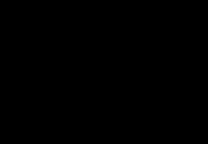
\includegraphics{figures/simple-gates}
\caption{(a) simple module output gate, (b) compound module output gate,
         (c) simple module input gate, (d) compound module input gate}
\label{fig:ch-simple-modules:gates}
\end{center}
\end{figure}

The start and end gates of the path can be found with the \ffunc{getPathStartGate()}
and \ffunc{getPathEndGate()} methods, which simply follow the \textit{previous gate} and
\textit{next gate} pointers, respectively, until they are \ttt{NULL}.

The \ffunc{isConnectedOutside()} and \ffunc{isConnectedInside()} methods
return whether a gate is connected on the outside or on the inside. They
examine either the \textit{previous} or the \textit{next} pointer, depending on the
gate type (input or output). For example, an output gate is \textit{connected outside}
if the \textit{next} pointer is non-\ttt{NULL}; the same function for an input gate
checks the \textit{previous} pointer. Again, see figure \ref{fig:ch-simple-modules:gates}
for an illustration.

The \ffunc{isConnected()} method is a bit different: it returns true if the gate
is \textit{fully} connected, that is, for a compound module gate
both inside and outside, and for a simple module gate, outside.

The following code prints the name of the gate a simple module gate is
connected to:

\begin{cpp}
cGate *gate = gate("somegate");
cGate *otherGate = gate->getType()==cGate::OUTPUT ? gate->getNextGate() :
                                                    gate->getPreviousGate();
if (otherGate)
  ev << "gate is connected to: " << otherGate->getFullPath() << endl;
else
  ev << "gate not connected" << endl;
\end{cpp}


\subsection{The Connection's Channel}

The channel object associated with a connection is accessible by
a pointer stored at the source gate of the connection. The pointer
is returned by the \ffunc{getChannel()} method of the gate:

\begin{cpp}
cChannel *channel = gate->getChannel();
\end{cpp}

The result may be \ttt{NULL}, that is, a connection may not have
an associated channel object.

If you have a channel pointer, you can get back its source gate
with the \ffunc{getSourceGate()} method:

\begin{cpp}
cGate *gate = channel->getSourceGate();
\end{cpp}

\cclass{cChannel} is just an abstract base class for channels, so
to access details of the channel you might need to cast the resulting
pointer into a specific channel class, for example \cclass{cDelayChannel}
or \cclass{cDatarateChannel}.

Another specific channel type is \cclass{cIdealChannel}, which basically
does nothing: it acts as if there was no channel object assigned to the
connection. {\opp} sometimes transparently inserts a \cclass{cIdealChannel}
into a channel-less connection, for example to hold the display string
associated with the connection.

Often you are not really interested in a specific connection's channel, but
rather in the \textit{transmission channel} (see
\ref{sec:simple-modules:packet-transmission}) of the connection path that
starts at a specific output gate. The transmission channel can be found by
following the connection path until you find a channel whose
\ffunc{isTransmissionChannel()} method returns \ttt{true}, but
\cclass{cGate} has a convenience method for this, named
\ffunc{getTransmissionChannel()}. An example usage:

\begin{cpp}
cChannel *txChan = gate("ppp$o")->getTransmissionChannel();
\end{cpp}

A complementer method to \ffunc{getTransmissionChannel()} is
\ffunc{getIncomingTransmissionChannel()}; it is usually invoked
on input gates, and searches the connection path in reverse direction.

\begin{cpp}
cChannel *incomingTxChan = gate("ppp$i")->getIncomingTransmissionChannel();
\end{cpp}

Both methods throw an error if no transmission channel is found. If this
is not suitable, use the similar \ffunc{findTransmissionChannel()} and
\ffunc{findIncomingTransmissionChannel()} methods that simply return
\ttt{NULL} in that case.

Channels are covered in more detail in section \ref{sec:simple-modules:channels}.


\section{Sending and Receiving Messages}
\label{sec:simple-modules:sending-and-receiving}

On an abstract level, an {\opp} simulation model is a set of
simple modules that communicate with each other via message passing.
The essence of simple modules is that they create, send, receive,
store, modify, schedule and destroy messages -- the rest of {\opp} exists
to facilitate this task, and collect statistics
about what was going on.

Messages in {\opp} are instances of the \cclass{cMessage} class or one of
its subclasses. Network packets are represented with \cclass{cPacket},
which is also subclassed from \cclass{cMessage}. Message objects are
created using the C++ \ttt{new} operator, and destroyed using the
\ttt{delete} operator when they are no longer needed.

Messages are described in detail in chapter \ref{cha:messages}.
At this point, all we need to know about them is that they are
referred to as \ttt{cMessage *} pointers. In the examples below,
messages will be created with \ttt{new cMessage("foo")} where
\ttt{"foo"} is a descriptive message name, used for visualization
and debugging purposes.


\subsection{Self-Messages}
\label{sec:ch-simple-modules:self-messages}

Nearly all simulation models need to schedule future events in order
to implement timers, timeouts, delays, etc. Some typical examples:

\begin{itemize}
  \item A source module that periodically creates and sends messages
    needs to schedule the next send after every send operation;
  \item A server which processes jobs from a queue needs to start
    a timer every time it begins processing a job. When the timer
    expires, the finished job can be sent out, and a new job may
    start processing;
  \item When a packet is sent by a communications protocol that employs
    retransmission, it needs to schedule a timeout so that the packet
    can be retransmitted if no acknowledge arrives within a certain
    amount of time.
\end{itemize}

In {\opp}, you solve such tasks by letting the simple module send a message
to itself; the message would be delivered to the simple module at a later
point of time. Messages used this way are called
\textit{self-messages}\index{self-message}, and the module class has
special methods for them that allow for implementing self-messages without
gates and connections.

\subsubsection{Scheduling an Event}

The module can send a message to itself using the \ffunc{scheduleAt()} function.
\ffunc{scheduleAt()} accepts an \textit{absolute} simulation time,
usually calculated as \ffunc{simTime()}+\textit{delta}:

\begin{cpp}
scheduleAt(absoluteTime, msg);
scheduleAt(simTime()+delta, msg);
\end{cpp}

Self-messages are delivered to the module in the same way as other
messages (via the usual receive calls or \ffunc{handleMessage()});
the module may call the \ffunc{isSelfMessage()} member of any received
message to determine if it is a self-message.

You can determine whether a message is currently in the FES\index{FES}
by calling its \ffunc{isScheduled()} member function.

\subsubsection{Cancelling an Event}

Scheduled self-messages can be cancelled\index{self-message!cancelling}
\index{message!cancelling} (i.e. removed from the FES\index{FES}).
This feature facilitates implementing timeouts.

\begin{cpp}
cancelEvent(msg);
\end{cpp}

The \ffunc{cancelEvent()} function takes a pointer to the message to
be cancelled, and also returns the same pointer. After having it
cancelled, you may delete the message or reuse it in subsequent
\ffunc{scheduleAt()} calls. \ffunc{cancelEvent()} has no effect if
the message is not scheduled at that time.

There is also a convenience method called \ffunc{cancelAndDelete()}
implemented as \ttt{if (msg!=NULL) delete cancelEvent(msg)};
this method is primarily useful for writing destructors.

The following example shows how to implement a timeout in a simple
imaginary stop-and-wait protocol. The code utilizes a \ttt{timeoutEvent}
module class data member that stores the pointer of the \cclass{cMessage} used
as self-message, and compares it to the pointer of the received message
to identify whether a timeout has occurred.

\begin{cpp}
void Protocol::handleMessage(cMessage *msg)
{
    if (msg == timeoutEvent) {
        // timeout expired, re-send packet and restart timer
        send(currentPacket->dup(), "out");
        scheduleAt(simTime() + timeout, timeoutEvent);
    }
    else if (...) {  // if acknowledgement received
        // cancel timeout, prepare to send next packet, etc.
        cancelEvent(timeoutEvent);
        ...
    }
    else {
       ...
    }
}
\end{cpp}


\subsubsection{Re-scheduling an Event}

If you want to reschedule an event which is currently scheduled to a different
simulation time, first you have to cancel it using \ffunc{cancelEvent()}.
This is shown in the following example code:

\begin{cpp}
if (msg->isScheduled())
    cancelEvent(msg);
scheduleAt(simTime() + delay, msg);
\end{cpp}


\subsection{Sending Messages}

Once created, a message object can be sent through an
output gate\index{output!gate} using one of the following functions:

\begin{cpp}
send(cMessage *msg, const char *gateName, int index=0);
send(cMessage *msg, int gateId);
send(cMessage *msg, cGate *gate);
\end{cpp}

In the first function, the argument \ttt{gateName} is the name of
the gate the message has to be sent through. If this gate is
a vector gate, \ttt{index} determines though which particular output
gate this has to be done; otherwise, the \ttt{index} argument is not
needed.

The second and third functions use the gate ID and the pointer to the gate
object. They are faster than the first one because they don't have to
search for the gate by name.

Examples:

\begin{cpp}
send(msg, "out");
send(msg, "outv", i); // send via a gate in a gate vector
\end{cpp}

To send via an inout gate, remember that an inout gate is an input and an
output gate glued together, and the two halves can be identified with the
\ttt{\$i} and \ttt{\$o} name suffixes. Thus, for sending you need to specify
the gate name with the \ttt{\$o} suffix:

\begin{cpp}
send(msg, "g$o");
send(msg, "g$o", i); // if "g[]" is a gate vector
\end{cpp}


\subsection{Broadcasts and Retransmissions}

When you implement broadcasts or retransmissions, two frequently
occurring tasks in protocol simulation, you might feel tempted
to use the same message in multiple \ffunc{send()} operations.
Do not do it -- you cannot send the same message object multiple times.
Instead, duplicate the message object.

Why? A message is like any real world object -- it cannot be at two places
at the same time. Once you've sent it, the message object no longer belongs
to the module: it is taken over by the simulation kernel, and will
eventually be delivered to the destination module. The sender module should
not even refer to its pointer any more. Once the message arrived in the
destination module, that module will have full authority over it -- it can
send it on, destroy it immediately, or store it for further handling. The
same applies to messages that have been scheduled -- they belong to the
simulation kernel until they are delivered back to the module.

To enforce the rules above, all message sending functions check that you
actually own the message you are about to send. If the message is in
another module, currently scheduled or in a queue, etc., you'll get a
runtime error: \textit{not owner of message}.
  \footnote{The feature does not increase runtime overhead significantly, because
  it uses the object ownership\index{ownership} management (described in
  Section \ref{sec:ch-sim-lib:ownership-management});
  it merely checks that the owner of the message is the module that
  wants to send it.}


\subsubsection{Broadcasting Messages}

In your model, you may need to broadcast a message to several destinations.
Broadcast can be implemented in a simple module by sending out copies
of the same message, for example on every gate of a gate vector.
As described above, you cannot use the same message pointer for
in all \ffunc{send()} calls -- what you have to do instead is
create copies (duplicates) of the message object and send them.

Example:

\begin{cpp}
for (int i=0; i<n; i++)
{
    cMessage *copy = msg->dup();
    send(copy, "out", i);
}
delete msg;
\end{cpp}

You might have noticed that copying the message for the last gate is
redundant: we can just send out the original message there.
Also, we can utilize gate IDs to avoid looking up the gate by name
for each send operation. We can exploit the fact that the ID of gate
$k$ in a gate vector can be produced as ${baseID} + k$.
The optimized version of the code looks like this:

\begin{cpp}
int outGateBaseId = gateBaseId("out");
for (int i=0; i<n; i++)
    send(i==n-1 ? msg : msg->dup(), outGateBaseId+i);
\end{cpp}


\subsubsection{Retransmissions}

Many communication protocols involve retransmissions of packets (frames).
When implementing retransmissions, you cannot just hold a pointer
to the same message object and send it again and again -- you'd get
the \textit{not owner of message} error on the first resend.

Instead, for (re)transmission, you should create and
send copies of the message, and retain the original.
When you are sure there will not be any more retransmission,
you can delete the original message.

Creating and sending a copy:

\begin{cpp}
// (re)transmit packet:
cMessage *copy = packet->dup();
send(copy, "out");
\end{cpp}

and finally (when no more retransmissions will occur):

\begin{cpp}
delete packet;
\end{cpp}


\subsection{Delayed Sending}
\label{sec:simple-modules:delayed-sending}

Sometimes it is necessary for module to hold a message for some time interval,
and then send it. This can be achieved with self-messages, but there is a
more straightforward method: delayed sending\index{delayed sending}. The
following methods are provided for delayed sending:

\begin{cpp}
sendDelayed(cMessage *msg, double delay, const char *gateName, int index);
sendDelayed(cMessage *msg, double delay, int gateId);
sendDelayed(cMessage *msg, double delay, cGate *gate);
\end{cpp}

The arguments are the same as for \ffunc{send()}, except for the extra
\textit{delay} parameter. The delay value must be non-negative.
The effect of the function is similar to as if the module
had kept the message for the delay interval and sent it afterwards;
even the \textit{sending time} timestamp of the message will be set to
the current simulation time plus \textit{delay}.

A example call:

\begin{cpp}
sendDelayed(msg, 0.005, "out");
\end{cpp}

The \ffunc{sendDelayed()} function does not internally perform a
\ffunc{scheduleAt()} followed by a \ffunc{send()}, but rather it computes
everything about the message sending up front, including the arrival time
and the target module. This has two consequences. First,
\ffunc{sendDelayed()} is more efficient than a \ffunc{scheduleAt()}
followed by a \ffunc{send()} because it eliminates one event. The second, less
pleasant consequence is that changes in the connection path during the
delay will \textit{not} be taken into account (because everything is
calculated in advance, before the changes take place).

\begin{note}
  The fact that \ffunc{sendDelayed()} computes the message arrival
  information up front does not make a difference if the model is static,
  but may lead to surprising results if the model changes in time.
  For example, if a connection in the path gets deleted, disabled, or
  reconnected to another module during the delay period, the message
  will still be delivered to the original module as if nothing happened.

  Therefore, despite its performance advantage, you should think twice
  before using \ffunc{sendDelayed()} in a simulation model. It may have
  its place in a one-shot simulation model that you know is static,
  but it certainly should be avoided in reusable modules that need to
  work correctly in a wide variety of simulation models.
\end{note}


\subsection{Direct Message Sending}
\label{sec:simple-modules:direct-sending}

At times it is covenient to be able to send a message directly to an input
gate of another module. The \ffunc{sendDirect()} function is provided for
this purpose.

This function has several flavors. The first set of \ffunc{sendDirect()}
functions accept a message and a target gate; the latter can be specified
in various forms:

\begin{cpp}
sendDirect(cMessage *msg, cModule *mod, int gateId)
sendDirect(cMessage *msg, cModule *mod, const char *gateName, int index=-1)
sendDirect(cMessage *msg, cGate *gate)
\end{cpp}

An example for direct sending:

\begin{cpp}
cModule *targetModule = getParentModule()->getSubmodule("node2");
sendDirect(new cMessage("msg"), targetModule, "in");
\end{cpp}

At the target module, there is no difference between messages received
directly and those received over connections.

The target gate must be an unconnected gate; in other words,
modules must have dedicated gates to be able to receive messages
sent via \ffunc{sendDirect()}. You cannot have a gate which receives
messages via both connections and \ffunc{sendDirect()}.

It is recommended to tag gates dedicated for receiving messages via
\ffunc{sendDirect()} with the \ttt{@directIn} property in the module's NED
declaration. This will cause {\opp} not to complain that the gate is not
connected in the network or compound module where the module is used.

An example:

\begin{ned}
simple Radio {
    gates:
        input radioIn @directIn; // for receiving air frames
}
\end{ned}

The target module is usually a simple module, but it can also be a compound
module. The message will follow the connections that start at the target
gate, and will be delivered to the module at the end of the path -- just as
with normal connections. The path must end in a simple module.

It is even permitted to send to an output gate, which will also cause the
message to follow the connections starting at that gate.
This can be useful, for example, when several submodules are sending
to a single output gate of their parent module.

A second set of \ffunc{sendDirect()} methods accept a propagation
delay and a transmission duration as parameters as well:

\begin{cpp}
sendDirect(cMessage *msg, simtime_t propagationDelay, simtime_t duration,
           cModule *mod, int gateId)
sendDirect(cMessage *msg, simtime_t propagationDelay, simtime_t duration,
           cModule *mod, const char *gateName, int index=-1)
sendDirect(cMessage *msg, simtime_t propagationDelay, simtime_t duration,
           cGate *gate)
\end{cpp}

The transmission duration parameter is important when the message is also
a packet (instance of \cclass{cPacket}). For messages that are not packets
(not subclassed from \cclass{cPacket}), the duration parameter
is ignored.

If the message is a packet, the duration will be written into the packet,
and can be read by the receiver with the \ffunc{getDuration()} method of
the packet.

The receiver module can choose whether it wants the simulation kernel
to deliver the packet object to it at the start or at the end of the
reception. The default is the latter; the module can change it by calling
\ffunc{setDeliverOnReceptionStart()} on the final input gate, that is, on
\ttt{targetGate->getPathEndGate()}.


\subsection{Packet Transmissions}
\label{sec:simple-modules:packet-transmission}

When a message is sent out on a gate, it usually travels through
a series of connections until it arrives at the destination module.
We call this series of connections a \textit{connection path}.

Several connections in the path may have an associated channel,
but there can be only one channel per path that models nonzero
transmission duration. This restriction is enforced by the simulation
kernel. This channel is called the \textit{transmission channel}.
  \footnote{Moreover, if \ffunc{sendDirect()} with a nonzero duration
  was used to send the packet to the start gate of the path,
  then the path cannot have a transmission channel at all.
  The point is that the a transission duration must be unambiguous.}

\begin{note}
  In practice, this means that there can be only one \ttt{ned.DatarateChannel}
  in the path. Note that unnamed channels with a \ttt{datarate} parameter
  also map to \ttt{ned.DatarateChannel}.
\end{note}

\subsubsection{Transmitting a Packet}

Packets may only be sent when the transmission channel is idle.
This means that after each transmission, the sender module needs
to wait until the channel has finished transmitting before it can
send another packet.

You can get a pointer to the transmission channel by calling the
\ffunc{getTransmissionChannel()} method on the output gate.
The channel's \ffunc{isBusy()} and \ffunc{getTransmissionFinishTime()}
methods can tell you whether a channel is currently transmitting,
and when the transmission is going to finish. (When the latter is
less or equal the current simulation time, the channel is free.)
If the channel is currently busy, sending needs to be postponed:
the packet can be stored in a queue, and a timer (self-message) can be
scheduled for the time when the channel becomes empty.

A code example to illustrate the above process:

\begin{cpp}
cPacket *pkt = ...; // packet to be transmitted
cChannel *txChannel = gate("out")->getTransmissionChannel();
simtime_t txFinishTime = txChannel->getTransmissionFinishTime();
if (txFinishTime <= simTime())
{
    // channel free; send out packet immediately
    send(pkt, "out");
}
else
{
    // store packet and schedule timer; when the timer expires,
    // the packet should be removed from the queue and sent out
    txQueue.insert(pkt);
    scheduleAt(txFinishTime, endTxMsg);
}
\end{cpp}

\begin{note}
  If there is a channel with a propagation delay in
  the path before the transmission channel, the delay should be manually
  substracted from the value returned by \ffunc{getTransmissionFinishTime()}!
  The same applies to \ffunc{isBusy()}: it tells whether the channel is
  currently busy, and not whether it will be busy when a packet that you send
  gets there. It is therefore advisable that you never use propagation delays
  in front of a transmission channel in a path.
\end{note}

The \ttt{getTransmissionChannel()} method searches the connection path each
time it is called. If performance is important, it is recommended that you
obtain the transmission channel pointer once, and cache it. When the network topology
changes, the cached channel pointer needs to be updated; section
\ref{sec:ch-simple-modules:model-change} describes the mechanism that can
be used to get notifications about topology changes.

\subsubsection{Receiving a Packet}

As a result of error modeling in the channel, the packet may arrive
with the \textit{bit error} flag set (\ffunc{hasBitError() method}.
It is the receiver module's responsibility to examine this flag
and take appropriate action (i.e. discard the packet).

Normally the packet object gets delivered to the destination module
at the simulation time that corresponds to finishing the reception
of the message (ie. the arrival of its last bit). However, the receiver
module may change this by ``reprogramming'' the receiver gate with
the \ffunc{setDeliverOnReceptionStart()} method:

\begin{cpp}
gate("in")->setDeliverOnReceptionStart(true);
\end{cpp}

This method may only be called on simple module input gates, and it
instructs the simulation kernel to deliver packets arriving through
that gate at the simulation time that corresponds to the
beginning of the reception process.
\ffunc{getDeliverOnReceptionStart()} only needs to be called once,
so it is usually done in the \ffunc{initialize()} method of the module.

\begin{figure}[htbp]
\begin{center}
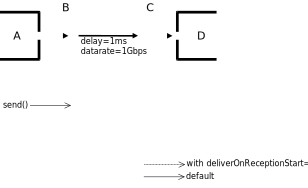
\includegraphics{figures/transmission}
\caption{Packet transmission}
\label{fig:ch-simple-modules:transmission}
\end{center}
\end{figure}

When a packet is delivered to the module, the packet's
\ffunc{isReceptionStart()} method can be called to determine
whether it corresponds to the start or end of the reception
process (it should be the same as the \ffunc{getDeliverOnReceptionStart()}
flag of the input gate), and \ffunc{getDuration()} returns the transmission
duration.

The following example code prints the start and end times of a packet reception:

\begin{cpp}
simtime_t startTime, endTime;
if (pkt->isReceptionStart())
{
    // gate was reprogrammed with setDeliverOnReceptionStart(true)
    startTime = pkt->getArrivalTime(); // or: simTime();
    endTime = startTime + pkt->getDuration();
}
else
{
    // default case
    endTime = pkt->getArrivalTime(); // or: simTime();
    startTime = endTime - pkt->getDuration();
}
ev << "interval: " << startTime << ".." << endTime << "\n";
\end{cpp}

Note that this works with wireless connections (\ffunc{sendDirect()})
as well; there, the duration is an argument to the \ffunc{sendDirect()}
call.

\subsubsection{Aborting Transmissions}

Sometimes you want the sender to abort transmission. The support {\opp}
provides for this task is the \ffunc{forceTransmissionFinishTime()} method
of channels. This method forcibly overwrites the \textit{transmissionFinishTime}
member of the channel with the given value, allowing the sender to transmit
another packet without raising the \textit{``channel is currently busy''}
error. The receiving party needs to be notified about the aborted transmission
by some user-defined means, for example by sending another packet
or an out-of-band message.

\subsubsection{Implementation of Message Sending}

Message sending is implemented like this: the arrival time\index{arrival time}
and the bit error\index{bit error} flag of a message are calculated right inside
the \ffunc{send()} call, then the message is inserted into the FES\index{FES}
with the calculated arrival time. The message does \textit{not} get scheduled
individually for each link. This implementation was chosen because of its
run-time efficiency.

\begin{note}
   The consequence of this implementation is that any change in the
   channel's parameters (delay, data rate, bit error rate, etc.) will only affect
   messages \textit{sent} after the change. Messages already underway will not
   be influenced by the change.

   This is not a huge problem in practice, but if it is important to model
   channels with changing parameters, the solution is to insert simple modules
   into the path to ensure strict scheduling.
\end{note}


\subsection{Receiving Messages with activity()}

\subsubsection{Receiving Messages}
\label{sec:simple-modules:receiving-messages}

\ffunc{activity()}-based modules receive messages with the \ffunc{receive()}
method of \cclass{cSimpleModule}. \ffunc{receive()} cannot be used with
\ffunc{handleMessage()}-based modules.

\begin{cpp}
cMessage *msg = receive();
\end{cpp}

The \ffunc{receive()} function accepts an optional \textit{timeout}
parameter\index{receive!timeout}. (This is a \textit{delta}, not an
absolute simulation time.) If no message arrives within the timeout
period, the function returns a \ttt{NULL} pointer.
    \footnote{Putaside-queue and the functions \ttt{receiveOn()},
    \ttt{receiveNew()}, and \ttt{receiveNewOn()} were deprecated
    in {\opp} 2.3 and removed in {\opp} 3.0.}

\begin{cpp}
simtime_t timeout = 3.0;
cMessage *msg = receive(timeout);

if (msg==NULL)
{
    ...   // handle timeout
}
else
{
    ...  // process message
}
\end{cpp}

\subsubsection{The wait() Function}
\label{sec:simple-modules:wait}

The \ffunc{wait()} function suspends the execution of the module for a
given amount of simulation time (a \textit{delta}). \ffunc{wait()} cannot
be used with \ffunc{handleMessage()}-based modules.

\begin{cpp}
wait(delay);
\end{cpp}

In other simulation software, \ffunc{wait()} is often called \textit{hold}.
Internally, the \ffunc{wait()} function is implemented by a
\ffunc{scheduleAt()} followed by a \ffunc{receive()}.
The \ffunc{wait()} function is very convenient in modules that do not need
to be prepared for arriving messages, for example message generators.
An example:

\begin{cpp}
for (;;)
{
    // wait for some, potentially random, amount of time, specified
    // in the interarrivalTime volatile module parameter
    wait(par("interarrivalTime").doubleValue());

    // generate and send message
    ...
}
\end{cpp}

It is a runtime error if a message arrives during the wait interval.
If you expect messages to arrive during the wait period, you can
use the \ffunc{waitAndEnqueue()} function. It takes a pointer to a queue object
(of class \cclass{cQueue}, described in chapter \ref{cha:the-simulation-library})
in addition to the wait interval. Messages that arrive during the
wait interval will be accumulated in the queue, so you can
process them after the \ffunc{waitAndEnqueue()} call returned.

\begin{cpp}
cQueue queue("queue");
...
waitAndEnqueue(waitTime, &queue);
if (!queue.empty())
{
    // process messages arrived during wait interval
    ...
}
\end{cpp}


\section{Channels}
\label{sec:simple-modules:channels}

\subsection{Overview}

Channels encapsulate parameters and behavior associated with connections.
Channel types are like simple modules, in the sense that they are declared
in NED, and there are C++ implementation classes behind them. Section
\ref{sec:ch-ned-lang:channels} describes NED language support for channels,
and explains how to associate C++ classes with channel types declared in
NED.

C++ channel classes must subclass from the abstract base class
\cclass{cChannel}. However, when creating a new channel class, it may be
more practical to extend one of the existing C++ channel classes behind the
three predefined NED channel types:

\begin{itemize}
  \item \cclass{cIdealChannel} implements the functionality of \ttt{ned.IdealChannel}
  \item \cclass{cDelayChannel} implements the functionality of \ttt{ned.DelayChannel}
  \item \cclass{cDatarateChannel} implements the functionality of \ttt{ned.DatarateChannel}
\end{itemize}

Channel classes need to be registered with the \fmac{Define\_Channel()} macro,
just like simple module classes need \fmac{Define\_Module()}.

The channel base class \cclass{cChannel} inherits from \cclass{cComponent},
so channels participate in the initialization and finalization protocol
(\ffunc{initialize()} and \ffunc{finish()}) described in
\ref{sec:simple-modules:initialize-and-finish}.

The parent module of a channel (as returned by the
\ffunc{getParentModule()}) is the module that contains
the connection. If a connection connects two modules that are children of
the same compound module, the channel's parent is the compound module. If
the connection connects a compound module to one of its submodules, the
channel's parent is also the compound module.


\subsection{The Channel API}

When subclassing \cclass{Channel}, you have to redefine and provide
implementations for the following pure virtual member functions:

\begin{itemize}
  \item \ffunc[isTransmissionChannel()]{bool isTransmissionChannel() const}
  \item \ffunc[getTransmissionFinishTime()]{simtime\_t getTransmissionFinishTime() const}
  \item \ffunc[processMessage()]{void processMessage(cMessage *msg, simtime\_t t, result\_t\& result)}
\end{itemize}

The first two functions are usually one-liners; the channel behavior is
encapsulated in the third function, \ffunc{processMessage()}.

\subsubsection{Transmission Channels}

The first function, \ffunc{isTransmissionChannel()}, determines whether
the channel is a \textit{transmission channel}, i.e. one that models
transmission duration. A transmission channel sets the duration field of
packets sent through it (see the \ffunc{setDuration()} field of
\cclass{cPacket}).

The \ffunc{getTransmissionFinishTime()} function is only used with
transmission channels, and it should return the simulation time the sender
will finish (or has finished) transmitting. This method is called by
modules that send on a transmission channel to find out when the channel
becomes available. The channel's \ffunc{isBusy()} method is implemented
simply as \ttt{return getTransmissionFinishTime() < simTime()}. For
non-transmission channels, the \ffunc{getTransmissionFinishTime()} return
value may be any simulation time which is less than or equal to the current
simulation time.

\subsubsection{The processMessage() Function}

The third function, \ffunc{processMessage()} encapsulates the channel's
functionality. However, before going into the details of this function
we need to understand how {\opp} handles message sending on connections.

Inside the \ffunc{send()} call, {\opp} follows the
connection path denoted by the \ffunc{getNextGate()} functions of gates,
until it reaches the target module. At each ``hop'', the corresponding
connection's channel (if the connection has one) gets a chance to add to
the message's arrival time (\textit{propagation time modeling}), calculate a
\textit{transmission duration}, and to modify the message object in various
ways, such as set the bit error flag in it (\textit{bit error modeling}).
After processing all hops that way, {\opp} inserts the message object
into the Future Events Set (FES\index{FES}, see section
\ref{sec:simple-modules:event-loop}), and the \ffunc{send()} call returns.
Then {\opp} continues to process events in increasing timestamp order.
The message will be delivered to the target module's \ffunc{handleMessage()}
(or \ffunc{receive()}) function when it gets to the front of the FES.

A few more details: a channel may instruct {\opp} to delete the message
instead of inserting it into the FES; this can be useful to model
disabled channels, or to model that the message has been lost altogether.
The \ffunc{getDeliverOnReceptionStart()} flag of the final gate in the path
will determine whether the transmission duration will be added to the
arrival time or not. Packet transmissions have been described in section
\ref{sec:simple-modules:packet-transmission}.

Now, back to the \ffunc{processMessage()} method.

The method gets called as part of the above process, when the message
is processed at the given hop. The method's arguments are the message
object, the simulation time the beginning of the message will reach
the channel (i.e. the sum of all previous propagation delays),
and a struct in which the method can return the results.

The \cclass{result\_t} struct is an inner type of \cclass{cChannel},
and looks like this:

\begin{cpp}
struct result_t {
    simtime_t delay;     // propagation delay
    simtime_t duration;  // transmission duration
    bool discard;        // whether the channel has lost the message
};
\end{cpp}

It also has a constructor that initializes all fields to zero; it is left
out for brevity.

The method should model the transmission of the given message starting at
the given \textit{t} time, and store the results (propagation delay,
transmission duration, deletion flag) in the result object. Only the
relevant fields in the result object need to be changed, others can be left
untouched.

Transmission duration and bit error modeling only applies to packets (i.e.
to instances of \cclass{cPacket}, where \cclass{cMessage}'s
\ffunc{isPacket()} returns true); it should be skipped for non-packet
messages. \ffunc{processMessage()} does not need to call the \ffunc{setDuration()}
method on the packet; this is done by the simulation kernel. However,
it should call \ffunc[setBitError()]{setBitError(true)} on the packet
if error modeling results in bit errors.

If the method sets the \ttt{discard} flag in the result object, that
means that the message object will be deleted by {\opp}; this facility
can be used to model that the message gets lost in the channel.

The \ffunc{processMessage()} method does not need to throw error on overlapping
transmissions, or if the packet's duration field is already set; these
checks are done by the simulation kernel before \ffunc{processMessage()} is called.

% TODO:
%
% \subsection{Active Channels}
%
% You may have noticed that channels subclasses from \cclass{cChannel} are
% passive in the sense that they cannot schedule events and cannot react
% to scheduled events. If you need such channels, use modules. Modules
% intented for use as channels should implement the \ttt{ned.IBidirectionalChannel}
% and \ttt{ned.IUnidirectionalChannel} NED interfaces. In future versions,
% {\opp} will be updated so that it handles such modules transparently
% as channels.
%
% XXX why no timers: efficiency. one can program simple modules that act like channels.


\subsection{Channel Examples}

To illustrate coding channel behavior, we look at how the built-in channel
types are implemented.

\cclass{cIdealChannel} lets through messages and packets without
any delay or change. Its \ffunc{isTransmissionChannel()} method returns
\ttt{false}, \ffunc{getTransmissionFinishTime()} returns $0s$, and the
body of its \ffunc{processMessage()} method is empty:

\begin{cpp}
void cIdealChannel::processMessage(cMessage *msg, simtime_t t, result_t& result)
{
}
\end{cpp}

\cclass{cDelayChannel} implements propagation delay, and it can be
disabled; in its disabled state, messages sent though it will be discarded.
This class still models zero transmission duration, so its
\ffunc{isTransmissionChannel()} and \ffunc{getTransmissionFinishTime()}
methods still return \ttt{false} and $0s$. The \ffunc{processMessage()} method
sets the appropriate fields in the \cclass{result\_t} struct:

\begin{cpp}
void cDelayChannel::processMessage(cMessage *msg, simtime_t t, result_t& result)
{
    // if channel is disabled, signal that message should be deleted
    result.discard = isDisabled;

    // propagation delay modeling
    result.delay = delay;
}
\end{cpp}

The \ffunc{handleParameterChange()} method is also redefined, so that
the channel can update its internal \ttt{delay} and \ttt{isDisabled}
data members if the corresponding channel parameters change during simulation.
\footnote{This code is a little simplified; the actual code uses a bit
in a bitfield to store the value of \ttt{isDisabled}.}

\cclass{cDatarateChannel} is different. It performs model packet duration
(duration is calculated from the data rate and the length of the packet),
so \ffunc{isTransmissionChannel()} returns \ttt{true}.
\ffunc{getTransmissionFinishTime()} returns the value of a \ttt{txfinishtime}
data member, which gets updated after every packet.

\begin{cpp}
simtime_t cDatarateChannel::getTransmissionFinishTime() const
{
    return txfinishtime;
}
\end{cpp}

\cclass{cDatarateChannel}'s \ffunc{processMessage()} method makes use of
the \ttt{isDisabled}, \ttt{datarate}, \ttt{ber} and \ttt{per} data
members, which are also kept up to date with the help of
\ffunc{handleParameterChange()}.

\begin{cpp}
void cDatarateChannel::processMessage(cMessage *msg, simtime_t t, result_t& result)
{
    // if channel is disabled, signal that message should be deleted
    if (isDisabled) {
        result.discard = true;
        return;
    }

    // datarate modeling
    if (datarate!=0 && msg->isPacket()) {
        simtime_t duration = ((cPacket *)msg)->getBitLength() / datarate;
        result.duration = duration;
        txfinishtime = t + duration;
    }
    else {
        txfinishtime = t;
    }

    // propagation delay modeling
    result.delay = delay;

    // bit error modeling
    if ((ber!=0 || per!=0) && msg->isPacket())
    {
        cPacket *pkt = (cPacket *)msg;
        if (ber!=0 && dblrand() < 1.0 - pow(1.0-ber, (double)pkt->getBitLength())
            pkt->setBitError(true);
        if (per!=0 && dblrand() < per)
            pkt->setBitError(true);
    }
}
\end{cpp}



\section{Stopping the Simulation}
\label{sec:simple-modules:stopping}

\subsection{Normal Termination}

You can finish the simulation with the \ffunc{endSimulation()} function:

\begin{cpp}
endSimulation();
\end{cpp}

\ffunc{endSimulation()} is rarely needed in practice because you
can specify simulation time and CPU time limits\index{simulation time limits}
in the ini file (see later).

\subsection{Raising Errors}

If your simulation encounters an error condition, you can throw a
\ttt{cRuntimeError} exception to terminate the simulation with
an error message (and in case of Cmdenv, a nonzero exit code).
The \ttt{cRuntimeError} class has a constructor whose argument list
is similar to \ffunc{printf()}:

\begin{cpp}
if (windowSize <= 0)
    throw cRuntimeError("Invalid window size %d; must be >=1", windowSize);
\end{cpp}

Do not include newline (\ttt{{\textbackslash}n}), period or exclamation mark
in the error text; it will be added by {\opp}.

You can achieve the same effect by calling the \ffunc{error()} method of
\cclass{cModule}

\begin{cpp}
if (windowSize <= 0)
    error("Invalid window size %d; must be >=1", windowSize);
\end{cpp}

Of course, the \ffunc{error()} method can only be used when a module pointer
is available.



\section{Finite State Machines}
\label{sec:simple-modules:fsm}

\subsubsection{Overview}

Finite State Machines\index{finite state machine} (FSMs)\index{FSM}
can make life with \ffunc{handleMessage()} easier. {\opp} provides a
class and a set of macros to build FSMs.

The key points are:
\begin{itemize}
\item{There are two kinds of states:
    \textit{transient}\index{transient states} and
    \textit{steady}\index{steady states}. On each event (that is, at
    each call to \ffunc{handleMessage()}), the FSM transitions out of
    the current (\textit{steady}) state, undergoes a series of state
    changes (runs through a number of \textit{transient} states), and
    finally arrives at another \textit{steady} state. Thus between two
    events, the system is always in one of the steady states.
    Transient states are therefore not really a must -- they exist
    only to group actions to be taken during a transition in a
    convenient way.}
\item{You can assign program code to handle entering and leaving a state
    (known as entry/exit code)\index{entry code}\index{exit code}.
    Staying in the same state is handled as leaving and re-entering
    the state.}
\item{Entry code should not modify the state (this is verified by
    {\opp}).  State changes (transitions) must be put into the exit
    code.}
\end{itemize}

{\opp}'s FSMs \textit{can} be nested\index{FSM!nested}. This means
that any state (or rather, its entry or exit code) may contain a
further full-fledged \fmac{FSM\_Switch()} (see below). This allows you
to introduce sub-states and thereby bring some structure into the
state space if it becomes too large.


\subsubsection{The FSM API}


FSM state is stored in an object of type \cclass{cFSM}. The possible states
are defined by an enum; the enum is also a place to define which
state is transient and which is steady. In the following example, SLEEP
and ACTIVE are steady states and SEND is transient (the numbers
in parentheses must be unique within the state type and they are used
for constructing the numeric IDs for the states):

\begin{cpp}
enum {
  INIT = 0,
  SLEEP = FSM_Steady(1),
  ACTIVE = FSM_Steady(2),
  SEND = FSM_Transient(1),
};
\end{cpp}



The actual FSM is embedded in a switch-like statement,
\fmac{FSM\_Switch()}, where you have cases for entering and leaving
each state:


\begin{cpp}
FSM_Switch(fsm)
{
  case FSM_Exit(state1):
    //...
    break;
  case FSM_Enter(state1):
    //...
    break;
  case FSM_Exit(state2):
    //...
    break;
  case FSM_Enter(state2):
    //...
    break;
  //...
};
\end{cpp}


State transitions\index{state transition} are done via calls to
\fmac{FSM\_Goto()}, which simply stores the new state in the
\cclass{cFSM} object:

\begin{cpp}
FSM_Goto(fsm, newState);
\end{cpp}

The FSM starts from the state with the numeric code 0; this state
is conventionally named INIT.


\subsubsection{Debugging FSMs}

FSMs can log their state transitions \ttt{ev}\index{ev},
with the output looking like this:

\begin{filelisting}
...
FSM GenState: leaving state SLEEP
FSM GenState: entering state ACTIVE
...
FSM GenState: leaving state ACTIVE
FSM GenState: entering state SEND
FSM GenState: leaving state SEND
FSM GenState: entering state ACTIVE
...
FSM GenState: leaving state ACTIVE
FSM GenState: entering state SLEEP
...
\end{filelisting}

To enable the above output, you have to \ttt{\#define FSM\_DEBUG}\index{FSM\_DEBUG}
before including \ttt{omnetpp.h}.

\begin{cpp}
#define FSM_DEBUG    // enables debug output from FSMs
#include <omnetpp.h>
\end{cpp}

The actual logging is done via the \fmac{FSM\_Print()} macro.
It is currently defined as follows, but you can change the
output format by undefining \ttt{FSM\_Print()} after including
\ffilename{omnetpp.ini} and providing a new definition instead.

\begin{cpp}
#define FSM_Print(fsm,exiting)
  (ev << "FSM " << (fsm).getName()
      << ((exiting) ? ": leaving state " : ": entering state ")
      << (fsm).getStateName() << endl)
\end{cpp}


\subsubsection{Implementation}


The \fmac{FSM\_Switch()} is a macro. It expands to a \ffunc{switch()}
statement embedded in a \ffunc{for()} loop which repeats until the
FSM\index{FSM} reaches a steady state. (The actual code is rather
scary, but if you are dying to see it, it is in \texttt{cfsm.h}.)

Infinite loops are avoided by counting state transitions: if
an FSM goes through 64 transitions without reaching a steady
state, the simulation will terminate with an error message.


\subsubsection{An Example}


Let us write another bursty packet generator. It will have two
states, SLEEP and ACTIVE. In the SLEEP state, the module does
nothing. In the ACTIVE state, it sends messages with a given
inter-arrival time. The code was taken from the Fifo2 sample
simulation.


\begin{cpp}
#define FSM_DEBUG
#include <omnetpp.h>

class BurstyGenerator : public cSimpleModule
{
  protected:
    // parameters
    double sleepTimeMean;
    double burstTimeMean;
    double sendIATime;
    cPar *msgLength;

    // FSM and its states
    cFSM fsm;
    enum {
      INIT = 0,
      SLEEP = FSM_Steady(1),
      ACTIVE = FSM_Steady(2),
      SEND = FSM_Transient(1),
    };

    // variables used
    int i;
    cMessage *startStopBurst;
    cMessage *sendMessage;

    // the virtual functions
    virtual void initialize();
    virtual void handleMessage(cMessage *msg);
};

Define_Module(BurstyGenerator);

void BurstyGenerator::initialize()
{
    fsm.setName("fsm");
    sleepTimeMean = par("sleepTimeMean");
    burstTimeMean = par("burstTimeMean");
    sendIATime = par("sendIATime");
    msgLength = &par("msgLength");
    i = 0;
    WATCH(i); // always put watches in initialize()
    startStopBurst = new cMessage("startStopBurst");
    sendMessage = new cMessage("sendMessage");
    scheduleAt(0.0,startStopBurst);
}

void BurstyGenerator::handleMessage(cMessage *msg)
{
   FSM_Switch(fsm)
   {
     case FSM_Exit(INIT):
       // transition to SLEEP state
       FSM_Goto(fsm,SLEEP);
       break;
     case FSM_Enter(SLEEP):
       // schedule end of sleep period (start of next burst)
       scheduleAt(simTime()+exponential(sleepTimeMean),
                  startStopBurst);
     break;
     case FSM_Exit(SLEEP):
       // schedule end of this burst
       scheduleAt(simTime()+exponential(burstTimeMean),
                  startStopBurst);
       // transition to ACTIVE state:
       if (msg!=startStopBurst) {
         error("invalid event in state ACTIVE");
       }
       FSM_Goto(fsm,ACTIVE);
       break;
     case FSM_Enter(ACTIVE):
       // schedule next sending
       scheduleAt(simTime()+exponential(sendIATime), sendMessage);
     break;
     case FSM_Exit(ACTIVE):
       // transition to either SEND or SLEEP
       if (msg==sendMessage) {
         FSM_Goto(fsm,SEND);
       } else if (msg==startStopBurst) {
         cancelEvent(sendMessage);
         FSM_Goto(fsm,SLEEP);
       } else {
         error("invalid event in state ACTIVE");
       }
       break;
     case FSM_Exit(SEND):
     {
       // generate and send out job
       char msgname[32];
       sprintf( msgname, "job-%d", ++i);
       ev << "Generating " << msgname << endl;
       cMessage *job = new cMessage(msgname);
       job->setBitLength( (long) *msgLength );
       job->setTimestamp();
       send( job, "out" );
       // return to ACTIVE
       FSM_Goto(fsm,ACTIVE);
       break;
     }
   }
}
\end{cpp}




\section{Navigating the Module Hierarchy}
\label{sec:simple-modules:walking-module-hierarchy}

\subsubsection{Module Vectors}


If a module is part of a module vector\index{module!vector}, the
\ffunc{getIndex()} and \ffunc{getVectorSize()} member functions can be used to
query its index and the vector size:

\begin{cpp}
ev << "This is module [" << module->getIndex() <<
      "] in a vector of size [" << module->size() << "].\n";
\end{cpp}


\subsubsection{Module IDs}


Each module in the network has a unique ID that is returned by the
\ffunc{getId()} member function. The module ID\index{module!id} is used
internally by the simulation kernel to identify modules.

\begin{cpp}
int myModuleId = getId();
\end{cpp}

If you know the module ID, you can ask the simulation object
(a global variable) to get back the module pointer:

\begin{cpp}
int id = 100;
cModule *mod = simulation.getModule( id );
\end{cpp}


Module IDs are guaranteed to be unique for the duration of the whole
simulation, even when modules are created and destroyed dynamically;
that is, IDs of deleted modules are not reused for newly created
modules.


\subsubsection{Walking Up and Down the Module Hierarchy}


The surrounding compound module can be accessed by the
\ffunc{getParentModule()} member function:

\begin{cpp}
cModule *parent = getParentModule();
\end{cpp}

For example, the parameters of the parent module are accessed
like this:

\begin{cpp}
double timeout = getParentModule()->par( "timeout" );
\end{cpp}


\cclass{cModule}'s \ffunc{findSubmodule()} and \ffunc{getSubmodule()}
member functions make it possible to look up the module's submodules
by name\index{module!submodule!lookup} (or name+index if the submodule
is in a module vector). The first one returns the numeric module ID of
the submodule, and the latter returns the module pointer.  If the
submodule is not found, they return -1 or NULL, respectively.

\begin{cpp}
int submodID = compoundmod->findSubmodule("child",5);
cModule *submod = compoundmod->getSubmodule("child",5);
\end{cpp}


The \ffunc{getModuleByRelativePath()} member function can be used to find
a submodule nested deeper than one level below. For example,

\begin{cpp}
compoundmod->getModuleByRelativePath("child[5].grandchild");
\end{cpp}

would give the same result as

\begin{cpp}
compoundmod->getSubmodule("child",5)->getSubmodule("grandchild");
\end{cpp}

(Provided that \ttt{child[5]} does exist, because otherwise the second
version would crash with an access violation because of the NULL
pointer dereference.)


The \cclass{cSimulation}::\ffunc{getModuleByPath()} function is similar
to \cclass{cModule}'s \ffunc{moduleByRelative\-Path()} function, and it
starts the search at the top-level module.


\subsubsection{Iterating over Submodules}


To access all modules within a compound module,
use \cclass{cSubModIterator}.

For example:

\begin{cpp}
for (cSubModIterator iter(*getParentModule()); !iter.end(); iter++)
{
  ev << iter()->getFullName();
}
\end{cpp}

(\ffunc{iter()} is pointer to the current module the iterator is at.)


The above method can also be used to iterate along a module
vector\index{module!vector!iteration}, since the \ffunc{getName()}
function returns the same for all modules:

\begin{cpp}
for (cSubModIterator iter(*getParentModule()); !iter.end(); iter++)
{
  if (iter()->isName(getName())) // if iter() is in the same
                              // vector as this module
  {
    int itsIndex = iter()->getIndex();
    // do something to it
  }
}
\end{cpp}


\subsubsection{Walking Along Links}

To determine the module at the other end of a connection, use
\cclass{cGate}'s \ffunc{getPreviousGate()}, \ffunc{getNextGate()} and
\ffunc{getOwnerModule()} functions. For example:

\begin{cpp}
cModule *neighbour = gate("out")->getNextGate()->getOwnerModule();
\end{cpp}

For input gates, you would use \ffunc{getPreviousGate()} instead of
\ffunc{getNextGate()}.


\section{Direct Method Calls Between Modules}
\label{sec:simple-modules:direct-method-calls}
\index{method calls!between modules}

In some simulation models, there might be modules which are too
tightly coupled for message-based communication to be efficient.
In such cases, the solution might be calling one simple module's public
C++ methods from another module.

Simple modules are C++ classes, so normal C++ method calls will
work. Two issues need to be mentioned, however:

\begin{itemize}
  \item how to get a pointer to the object representing the module;
  \item how to let the simulation kernel know that a method call across modules
     is taking place.
\end{itemize}

Typically, the called module is in the same compound module as the caller,
so the \ffunc{getParentModule()} and \ffunc{getSubmodule()} methods of
\cclass{cModule} can be used to get a \ttt{cModule*} pointer to the
called module. (Further ways to obtain the pointer are described
in the section \ref{sec:simple-modules:walking-module-hierarchy}.)
The \ttt{cModule*} pointer then has to be cast to the actual C++ class
of the module, so that its methods become visible.

This makes the following code:

\begin{cpp}
cModule *calleeModule = getParentModule()->getSubmodule("callee");
Callee *callee = check_and_cast<Callee *>(calleeModule);
callee->doSomething();
\end{cpp}

The \ffunc{check\_and\_cast<>()} template function on the second line
is part of {\opp}. It performs a standard C++ \ttt{dynamic\_cast},
and checks the result: if it is NULL, \ttt{check\_and\_cast} raises an {\opp} error.
Using \ttt{check\_and\_cast} saves you from writing error checking
code: if \ttt{calleeModule} from the first line is NULL because
the submodule named \ttt{"callee"} was not found, or if that
module is actually not of type \ttt{Callee}, an error is thrown
from \ttt{check\_and\_cast}.

The second issue is how to let the simulation kernel know that
a method call across modules is taking place. Why is this necessary
in the first place? First, the simulation kernel always has to know which
module's code is currently executing, in order for ownership handling
and other internal mechanisms to work correctly. Second, the Tkenv
simulation GUI can animate method calls, but to be able to do that,
it has to know about them. Third, method calls are also recorded
in the event log.

The solution is to add the \ttt{Enter\_Method()} or \ttt{Enter\_Method\_Silent()}
macro at the top of the methods that may be invoked from other
modules. These calls perform context switching, and, in case of
\ttt{Enter\_Method()}, notify the simulation GUI so that animation
of the method call can take place. \ttt{Enter\_Method\_Silent()}
does not animate the method call, but otherwise it is equivalent
\ttt{Enter\_Method()}. Both macros accept a \ttt{printf()}-like
argument list (it is optional for \ttt{Enter\_Method\_Silent()}),
which should produce a string with the method name and the
actual arguments as much as practical. The string is displayed in
the animation (\ttt{Enter\_Method()} only) and recorded into the event log.


\begin{cpp}
void Callee::doSomething()
{
    Enter_Method("doSomething()");
    ...
}
\end{cpp}



\section{Dynamic Module Creation}
\label{sec:simple-modules:dynamic-module-creation}
\index{module!dynamic creation}

\subsection{When Do You Need Dynamic Module Creation}

In some situations you need to dynamically create and maybe destroy
modules. For example, when simulating a mobile network,
you may create a new module whenever a new user enters
the simulated area, and dispose of them when they leave the area.

As another example, when implementing a server or a transport
protocol, it might be convenient to dynamically create modules
to serve new connections, and dispose of them when the connection
is closed. (You would write a manager module that receives connection
requests and creates a module for each connection.
The Dyna example simulation does something like this.)

Both simple and compound modules can be created dynamically.
If you create a compound module, all its submodules will be created
recursively.

It is often convenient to use direct message sending with dynamically
created modules.

Once created and started, dynamic modules aren't any different from
``static'' modules; for example, one could also delete static modules
during simulation (though it is rarely useful.)


\subsection{Overview}


To understand how dynamic module creation works, you have to know a
bit about how {\opp} normally instantiates modules. Each module type
(class) has a corresponding factory object of the class
\cclass{cModuleType}. This object is created under the hood by the
\fmac{Define\_Module()} macro, and it has a factory
method which can instantiate the module class (this function basically
only consists of a \ttt{return new \textit{<moduleclass>}(...)} statement).

The \cclass{cModuleType} object can be looked up by its name
string (which is the same as the module class name). Once you have its
pointer, it is possible to call its factory method and create an
instance of the corresponding module class -- without having to
include the C++ header file containing module's class declaration
into your source file.

The \cclass{cModuleType} object also knows what gates and
parameters the given module type has to have. (This info comes from
NED files.)

Simple modules can be created in one step. For a compound module, the
situation is more complicated, because its internal structure
(submodules, connections) may depend on parameter values and gate
vector sizes. Thus, for compound modules it is generally required to
first create the module itself, second, set parameter values and gate
vector sizes, and then call the method that creates its submodules and
internal connections.

As you know already, simple modules with \ffunc{activity()} need a
starter message\index{starter messages}. For statically created
modules, this message is created automatically by {\opp}, but for
dynamically created modules, you have to do this explicitly by calling
the appropriate functions.

Calling \ffunc{initialize()} has to take place after insertion of the
starter messages, because the initializing code may insert new messages
into the FES\index{FES}, and these messages should be processed
\textit{after} the starter message.


\subsection{Creating Modules}

The first step is to find the factory object. The \ttt{cModuleType::get()}
function expects a fully qualified NED type name, and returns the factory
object:

\begin{cpp}
cModuleType *moduleType = cModuleType::get("foo.nodes.WirelessNode");
\end{cpp}

The return value does not need to be checked for \ttt{NULL}, because
the function raises an error if the requested NED type was not found.
(If this behavior is not what you need, you can use the similar
\ttt{cModuleType::find()} function, which returns \ttt{NULL} if the type
was not found.)

\subsubsection{The All-in-One Method}

\cclass{cModuleType} has a \ffunc[createScheduleInit()]{createScheduleInit(const
char *name, cModule *parentmod)} convenience function to get a module up
and running in one step.

\begin{cpp}
cModule *mod = moduleType->createScheduleInit("node", this);
\end{cpp}

\ffunc{createScheduleInit()} performs the following steps: \ffunc{create()},
\ffunc{finalizeParameters()}, \ffunc{buildInside()},
\ffunc[scheduleStart()]{scheduleStart(now)} and \ffunc{callInitialize()}.

This method can be used for both simple and compound modules. Its
applicability is somewhat limited, however: because it does everything in
one step, you do not have the chance to set parameters or gate sizes, and
to connect gates before \ffunc{initialize()} is called.
(\ffunc{initialize()} expects all parameters and gates to be in place and
the network fully built when it is called.) Because of the above
limitation, this function is mainly useful for creating basic simple
modules.


\subsubsection{The Detailed Procedure}

If the \ffunc{createScheduleInit()} all-in-one method is not applicable,
one needs to use the full procedure. It consists of five steps:

\begin{enumerate}
  \item Find the factory object;
  \item Create the module;
  \item Set up its parameters and gate sizes as needed;
  \item Tell the (possibly compound) module to recursively create
        its internal submodules and connections;
  \item Schedule activation message(s) for the new simple module(s).
\end{enumerate}

Each step (except for Step 3.) can be done with one line of code.

See the following example, where Step 3 is omitted:

\begin{cpp}
// find factory object
cModuleType *moduleType = cModuleType::get("foo.nodes.WirelessNode");

// create (possibly compound) module and build its submodules (if any)
cModule *module = moduleType->create("node", this);
module->finalizeParameters();
module->buildInside();

// create activation message
module->scheduleStart(simTime());
\end{cpp}

If you want to set up parameter values or gate vector sizes (Step 3.),
the code goes between the \ffunc{create()} and
\ffunc{buildInside()} calls:

\begin{cpp}
// create
cModuleType *moduleType = cModuleType::get("foo.nodes.WirelessNode");
cModule *module = moduleType->create("node", this);

// set up parameters and gate sizes before we set up its submodules
module->par("address") = ++lastAddress;
module->finalizeParameters();

module->setGateSize("in", 3);
module->setGateSize("out", 3);

// create internals, and schedule it
module->buildInside();
module->scheduleStart(simTime());
\end{cpp}


\subsection{Deleting Modules}

To delete a module dynamically\index{module!dynamic deletion}, use
\cclass{cModule}'s \ffunc{deleteModule()} member function:

\begin{cpp}
module->deleteModule();
\end{cpp}

If the module was a compound module, this involves recursively
deleting all its submodules. A simple module can also delete itself;
in this case, the \ffunc{deleteModule()} call does not return to the
caller.

Currently, you cannot safely delete a compound module from a simple module
in it; you must delegate the job to a module outside the compound
module.


\subsection{Module Deletion and finish()}

\ffunc{finish()} is called for \textit{all} modules at the end of the
simulation, no matter how the modules were created. If a module is
dynamically deleted before that, \ffunc{finish()} will not be invoked
(\ffunc{deleteModule()} does not do it). However, you can still manually
invoke it before \ffunc{deleteModule()}.

You can use the \ffunc{callFinish()} function to invoke \ffunc{finish()}
(It is not a good idea to invoke \ffunc{finish()} directly). If you are
deleting a compound module, \ffunc{callFinish()} will recursively invoke
\ffunc{finish()} for all submodules, and if you are deleting a simple
module from another module, \ffunc{callFinish()} will do the context switch
for the duration of the call.
  \footnote{The \ffunc{finish()} function has even been made \ttt{protected}
  in \cclass{cSimpleModule}, in order to discourage its invocation from
  other modules.}

Example:

\begin{cpp}
mod->callFinish();
mod->deleteModule();
\end{cpp}


\subsection{Creating Connections}
\index{connection!creating}

Connections can be created using \cclass{cGate}'s \ffunc{connectTo()}
method.
  \footnote{The earlier \ffunc{connect()} global functions that
  accepted two gates have been deprecated, and may be removed
  from further {\opp} releases.}
\ffunc{connectTo()} should be invoked on the source gate
of the connection, and expects the destination gate pointer as
an argument:

\begin{cpp}
srcGate->connectTo(destGate);
\end{cpp}

The \textit{source} and \textit{destination} words correspond
to the direction of the arrow in NED files.

As an example, we create two modules and connect them in both directions:

\begin{cpp}
cModuleType *moduleType = cModuleType::get("TicToc");
cModule *a = modtype->createScheduleInit("a", this);
cModule *b = modtype->createScheduleInit("b", this);

a->gate("out")->connectTo(b->gate("in"));
b->gate("out")->connectTo(a->gate("in"));
\end{cpp}

\ffunc{connectTo()} also accepts a channel object (\ttt{cChannel*}) as an
additional, optional argument. Similarly to modules, channels can be
created using their factory object of the type \cclass{cChannelType}:

\begin{cpp}
cGate *outg=..., *ing=...;

// find factory object and create a channel
cChannelType *channelType = cChannelType::get("foo.util.Channel");
cChannel *channel = channelType->create("channel");

// create connecting
outg->connectTo(ing, channel);
\end{cpp}

The channel object will be owned by the source gate of the connection, and
you cannot reuse the same channel object with several connections.

If you need one of the built-in channel types (\cclass{cIdealChannel},
\cclass{cDelayChannel} or \cclass{cDatarateChannel}), the step to find the
factory object can be spared, as those classes have static \ffunc{create()}
functions to create a channel instance.

\cclass{cDatarateChannel} also has member functions to set up its
parameters: \ffunc{setDelay()}, \ffunc{setBitErrorRate()},
\ffunc{setPacketErrorRate()} and \ffunc{setDatarate()}.

An example that sets up a channel with a delay:

\begin{cpp}
cDatarateChannel *channel = cDatarateChannel::create("channel");
channel->setDelay(0.001);

a->gate("out")->connectTo(b->gate("in"), channel); // a, b are modules
\end{cpp}


\subsection{Removing Connections}
\index{connection!removing}

The \ffunc{disconnect()} method of \cclass{cGate} can be
used to remove connections. This method has to be invoked
on the \textit{source} side of the connection. It also destroys
the channel object associated with the connection, if one has been set.

\begin{cpp}
srcGate->disconnect();
\end{cpp}

\section{Signals}
\label{sec:simple-modules:signals}

This section describes \textit{simulation signals}, or signals for short.
Signals are a versatile concept that first appeared in {\opp} 4.1.

Simulation signals can be used for:

\begin{itemize}
  \item exposing statistical properties of the model, without specifying
        whether and how to record them
  \item receiving notifications about simulation model changes at runtime, and
        acting upon them
  \item implementing a publish-subscribe style communication among modules;
        this is advantageous when the producer and consumer of the information
        do not know about each other, and possibly there is many-to-one or
        many-to-many relationship among them
  \item emitting information for other purposes, for example as input for
        custom animation effects
\end{itemize}

Signals are emitted by components (modules and channels). Signals propagate
on the module hierarchy up to the root. At any level, one can register
listeners (callback objects); these listeners will be notified (called
back) whenever a signal value is emitted. The result of upwards propagation
is that listeners registered at a compound module can receive signals from
all components in that submodule tree. A listener registered at the system
module can receive signals from the whole simulation.

\begin{note}
    A channel's parent is the (compound) module that contains the connection,
    not the owner of either gate the channel is connected to.
\end{note}

Signals are identified by signal names (i.e. strings), but for efficiency reasons
at runtime we use dynamically assigned numeric identifiers (signal IDs,
typedef'd as \ttt{simsignal\_t}). The mapping of signal names to signal IDs is
global, so all modules and channels asking to resolve a particular signal name
will get back the same numeric signal ID.

Listeners can subscribe to signal names or IDs, regardless of their
source. For example, if two different and unrelated module types, say
\ttt{Queue} and \ttt{Buffer}, both emit a signal named \ttt{"length"}, then
a listener that subscribes to \ttt{"length"} at some higher compound module
will get notifications from both \ttt{Queue} and \ttt{Buffer} module
instances. The listener can still look at the source of the signal if it
wants to distinguish the two (it is available as a parameter to the
callback function), but the signals framework itself does not have such a
feature.

\begin{note}
  Because the component type that emits the signal is not part of the signal's
  identity, it is advised to choose signal names carefully. A good naming scheme
  facilitates "merging" of signals that arrive from different sources but
  mean the same thing, and reduces the chance of collisions between signals that
  accidentally have the same name but represent different things.
\end{note}

When a signal is emitted, it can carry a value with it. This is realized via
overloaded \ffunc{emit()} methods in components, and overloaded \ffunc{receiveSignal()}
methods in listeners. The signal value can be of selected primitive types, or an
object pointer; anything that is not feasible to emit as a primitive type may be
wrapped into an object, and emitted as such.

\subsection{Design Considerations and Rationale}

The implementation of signals is based on the following assumptions:

\begin{itemize}
  \item subscribe/unsubscribe operations are rare compared to \ffunc{emit()}
    calls, so it is \ffunc{emit()} that needs to be efficient
  \item the signals mechanism is present in every module, so per-module
    memory overhead must be kept as low as possible
  \item it is expected that modules and channels will be heavily instrumented
    with signals, and only a subset of signals will actually be used
    (will have listeners) in any particular simulation; therefore,
    the CPU and memory overhead of momentarily unused signals must be
    as low as possible
\end{itemize}

These goals have been achieved in the 4.1 version with the following
implementation. First, the data structure that used to store listeners in
components is dynamically allocated, so if there are no listeners, the
per-component overhead is only the size of the pointer (which will be
\ttt{NULL} then).

Second, additionally there are two bitfields in every component that store
which one of the first 64 signals (IDs 0..63) have local listeners and
listeners in ancestor modules.\footnote{It is assumed that there will be
typically less than 64 frequently used signals used at a time in a
simulation.} Using these bitfields, it is possible to determine in constant
time for the first 64 signals whether the signal has listeners, so
\ffunc{emit()} can return immediately if there are none. For other signals,
\ffunc{emit()} needs to examine the listener lists up to the root every
time. Even if a simulation uses more than 64 signals, in
performance-critical situations it is possible to arrange that frequently
emitted signals (e.g. \ttt{"txBegin"}) get the ``fast'' signal IDs, while
infrequent signals (like e.g. \ttt{"routerDown"}) get the rest.


\subsection{The Signals Mechanism}
\label{sec:simple-modules:signals-api}

Signal-related methods are declared on \cclass{cComponent}, so they are available
for both \cclass{cModule} and \cclass{cChannel}.

\subsubsection{Signal IDs}

Signals are identified by names, but internally numeric signal IDs are used
for efficiency. The \ffunc{registerSignal()} method takes a signal name as
parameter, and returns the corresponding \ttt{simsignal\_t} value.
The method is static, illustrating the fact that signal names are global.
An example:

\begin{cpp}
simsignal_t lengthSignalId = registerSignal("length");
\end{cpp}

The \ffunc{getSignalName()} method (also static) does the reverse:
it accepts a \ttt{simsignal\_t}, and returns the name of the signal as
\ttt{const char *} (or \ttt{NULL} for invalid signal handles):

\begin{cpp}
const char *signalName = getSignalName(lengthSignalId); // --> "length"
\end{cpp}

\begin{note}
  Since {\opp} 4.3, the lifetime of signal IDs is the entire program, and
  it is possible to call \ffunc{registerSignal()} from initializers of
  global variables, e.g. static class members. In earlier versions,
  signal IDs were usually allocated in \ffunc{initialize()}, and were
  only valid for that simulation run.
\end{note}

\subsubsection{Emitting Signals}

The \ffunc{emit()} family of functions emit a signal from the module or
channel. They take two parameters, the signal ID (\ttt{simsignal\_t}) and
the value:

\begin{cpp}
emit(lengthSignalId, queue.length());
\end{cpp}

The value can be of type \ttt{long}, \ttt{double}, \ttt{simtime\_t},
\ttt{const char *}, or \ttt{cObject *}. Other types can be cast into
one of these types, or wrapped into an object subclassed from \ttt{cObject}.

When there are no listeners, the runtime cost of \ttt{emit()} is usually minimal.
However, if producing a value has a significant runtime cost, then the
\ffunc{mayHaveListeners()} or \ffunc{hasListeners()} method can be used
to check beforehand whether the given signal has any listeners at all --
if not, emitting the signal can be skipped. For some signals (in {\opp} 4.3,
the first 64 signals used), the information whether it has listeners is cached per
component, and can be produced in constant time.

Example usage:

\begin{cpp}
if (mayHaveListeners(distanceToTargetSignal))
{
    double d = sqrt((x-targetX)*(x-targetX) + (y-targetY)*(y-targetY));
    emit(distanceToTargetSignal, d);
}
\end{cpp}

The \ffunc{mayHaveListeners()} method is very efficient (a constant-time
operation) because it only uses this cached information; if the state is
not cached for the signal, it just returns \ttt{true}. In contrast,
\ffunc{hasListeners()} will search up to the top of the module tree if
the answer is not cached, so it is generally slower. We recommend that
you take into account the cost of producing notification information when
deciding between \ffunc{mayHaveListeners()} and \ffunc{hasListeners()}.


\subsubsection{Signal Data Objects}

When emitting a signal with a \ttt{cObject*} pointer, you can pass as data
an object that you already have in the model, provided you have a suitable
object at hand. However, it is often necessary to declare a custom class
to hold all the details, and fill in an instance just for the purpose of
emitting the signal.

The custom notification class must be derived from \cclass{cObject}.
We recommend that you also add \cclass{noncopyable} as a base class, because
then you don't need to write a copy constructor, assignment operator, and
\ffunc{dup()} function, sparing some work. When emitting the signal, you
can create a temporary object, and pass its pointer to the \ffunc{emit()}
function.

An example of custom notification classes is the firing of model change notifications
(see \ref{sec:ch-simple-modules:model-change}). The data class
that accompanies a signal that announces that a gate or gate vector is
about to be created looks like this:

\begin{cpp}
class cPreGateAddNotification : public cObject, noncopyable
{
  public:
    cModule *module;
    const char *gateName;
    cGate::Type gateType;
    bool isVector;
};
\end{cpp}

And the code that emits the signal:

\begin{cpp}
if (hasListeners(PRE_MODEL_CHANGE))
{
    cPreGateAddNotification tmp;
    tmp.module = this;
    tmp.gateName = gatename;
    tmp.gateType = type;
    tmp.isVector = isVector;
    emit(PRE_MODEL_CHANGE, &tmp);
}
\end{cpp}


\subsubsection{Subscribing to Signals}

The \ffunc{subscribe()} method registers a listener for a signal.
Listeners are objects that extend the \cclass{cIListener} class.
The same listener object can be subscribed to multiple signals.
\ffunc{subscribe()} has two arguments: the signal and a pointer to
the listener object:

\begin{cpp}
cIListener *listener = ...;
simsignal_t lengthSignalId = registerSignal("length");
subscribe(lengthSignalId, listener);
\end{cpp}

For convenience, the \ffunc{subscribe()} method has a variant
that takes the signal name directly, so the \ffunc{registerSignal()}
call can be omitted:

\begin{cpp}
cIListener *listener = ...;
subscribe("length", listener);
\end{cpp}

One can also subscribe at other modules, not only the local one.
For example, in order to get signals from all parts of the model,
one can subscribe at the system module level:

\begin{cpp}
cIListener *listener = ...;
simulation.getSystemModule()->subscribe("length", listener);
\end{cpp}

The \ffunc{unsubscribe()} method has the same parameter list
as \ffunc{subscribe()}, and unregisters the given listener
from the signal:

\begin{cpp}
unsubscribe(lengthSignalId, listener);
\end{cpp}

or

\begin{cpp}
unsubscribe("length", listener);
\end{cpp}

It is an error to subscribe the same listener to the same
signal twice.

\begin{note}
  When a listener is deleted, it must already be unsubscribed from
  all components it has subscribed to. This is explained in
  \ref{sec:simple-modules:signals:life-cycle}.
\end{note}

It is possible to test whether a listener is subscribed to a signal,
using the \ffunc{isSubscribed()} method which also takes the same
parameter list.

\begin{cpp}
if (isSubscribed(lengthSignalId, listener))
{
    ...
}
\end{cpp}

For completeness, there are methods for getting the list of signals
that the component has subscribed to (\ffunc{getLocalListenedSignals()}),
and the list of listeners for a given signal (\ffunc{getLocalSignalListeners()}).
The former returns \ttt{std::vector<simsignal\_t>}; the latter takes
a signal ID (\ttt{simsignal\_t}) and returns \ttt{std::vector<cIListener*>}.

The following example prints the number of listeners for each signal:

\begin{cpp}
EV << "Signal listeners:\n";
std::vector<simsignal_t> signals = getLocalListenedSignals();
for (unsigned int i = 0; i < signals.size(); i++) {
    simsignal_t signalID = signals[i];
    std::vector<cIListener*> listeners = getLocalSignalListeners(signalID);
    EV << getSignalName(signalID) << ": " << listeners.size() << " signals\n";
}
\end{cpp}

\subsubsection{Listeners}

Listeners are objects that subclass from the \cclass{cIListener} class, which
declares the following methods:

\begin{cpp}
class cIListener
{
  public:
    virtual ~cIListener() {}
    virtual void receiveSignal(cComponent *src, simsignal_t id, long l) = 0;
    virtual void receiveSignal(cComponent *src, simsignal_t id, double d) = 0;
    virtual void receiveSignal(cComponent *src, simsignal_t id, simtime_t t) = 0;
    virtual void receiveSignal(cComponent *src, simsignal_t id, const char *s) = 0;
    virtual void receiveSignal(cComponent *src, simsignal_t id, cObject *obj) = 0;
    virtual void finish(cComponent *component, simsignal_t id) {}
    virtual void subscribedTo(cComponent *component, simsignal_t id) {}
    virtual void unsubscribedFrom(cComponent *component, simsignal_t id) {}
};
\end{cpp}

This class has a number of virtual methods:

\begin{itemize}
  \item Several overloaded \ffunc{receiveSignal()} methods, one for each
    data type. Whenever a signal is emitted (via \ffunc{emit()}),
    the matching \ffunc{receiveSignal()} methods of subscribed listeners
    are invoked.
  \item \ffunc{finish()} is called by a component on its local listeners
    after the component's \ffunc{finish()} method was called. If the listener
    is subscribed to multiple signals or at multiple components, the method
    will be called multiple times. Note that \ffunc{finish()} methods in general
    are not invoked if the simulation terminates with an error, so this method
    is not a place for doing cleanup.
  \item \ffunc{subscribedTo()}, \ffunc{unsubscribedFrom()} are called
    when this listener object is subscribed/unsubscribed to (from) a signal.
    These methods give the opportunity for listeners to track whether
    and where they are subscribed. It is also OK for a listener to delete
    itself in the last statement of the \ffunc{unsubscribedFrom()} method,
    but you must be sure that there are no other places the same listener
    is still subscribed.
\end{itemize}

Since \cclass{cIListener} has a large number of pure virtual methods, it is more
convenient to subclass from \cclass{cListener}, a do-nothing implementation
instead. It defines \ffunc{finish()}, \ffunc{subscribedTo()} and
\ffunc{unsubscribedFrom()} with an empty body, and the \ffunc{receiveSignal()}
methods with a bodies that throw a \ttt{"Data type not supported"} error.
You can redefine the \ffunc{receiveSignal()} method(s) whose data type
you want to support, and signals emitted with other (unexpected) data
types will result in an error instead of going unnoticed.

The order in which listeners will be notified is undefined (it is not necessarily
the same order in which listeners were subscribed.)

\subsubsection{Listener Life Cycle}
\label{sec:simple-modules:signals:life-cycle}

When a component (module or channel) is deleted, it automatically
unsubscribes (but does not delete) the listeners it has. When a
module is deleted, it first unsubscribes all listeners from all
modules and channels in its submodule tree before starting
to recursively delete the modules and channels themselves.

When a listener is deleted, it must already be unsubscribed from all
components at that point. If it is not unsubscribed, pointers to the dead
listener object will be left in the components' listener lists, and the
components will crash inside an \ffunc{emit()} call, or when they
try to invoke \ffunc{unsubscribedFrom()} on the dead listener from their
destructors. The \cclass{cIListener} class contains a subscription count,
and prints a warning message when it is not zero in the destructor.

\begin{note}
  If your module has added listeners to other modules (e.g. the toplevel
  module), these listeners must be unsubscribed in the module
  destructor at latest. Remember to make sure the modules still exist before you
  call \ffunc{unsubscribe()} on them, unless they are an ancestor
  of your module in the module tree.
\end{note}


\subsection{Listening to Model Changes}
\label{sec:ch-simple-modules:model-change}

In simulation models it is often useful to hold references to other
modules, a connecting channel or other objects, or to cache information
derived from the model topology. However, such pointers or data may
become invalid when the model changes at runtime, and need to be updated
or recalculated. The problem is how to get notification that something has
changed in the model.

\begin{note}
  Whenever you see a \ttt{cModule*}, \ttt{cChannel*}, \ttt{cGate*} or
  similar pointer kept as state in a simple module, you should think about
  how it will be kept up-to-date if the model changes at runtime.
\end{note}

The solution is, of course, signals. {\opp} has two built-in signals,
\fmac{PRE\_MODEL\_CHANGE} and \fmac{POST\_MODEL\_CHANGE} (these macros
are \ttt{simsignal\_t} values, not names) that are emitted before and
after each model change.

Pre/post model change notifications are emitted with data objects that
carry the details of the change. The data classes are:

\begin{itemize}
  \item \cclass{cPreModuleAddNotification} / \cclass{cPostModuleAddNotification}
  \item \cclass{cPreModuleDeleteNotification} / \cclass{cPostModuleDeleteNotification}
  \item \cclass{cPreModuleReparentNotification} / \cclass{cPostModuleReparentNotification}
  \item \cclass{cPreGateAddNotification} / \cclass{cPostGateAddNotification}
  \item \cclass{cPreGateDeleteNotification} / \cclass{cPostGateDeleteNotification}
  \item \cclass{cPreGateVectorResizeNotification} / \cclass{cPostGateVectorResizeNotification}
  \item \cclass{cPreGateConnectNotification} / \cclass{cPostGateConnectNotification}
  \item \cclass{cPreGateDisconnectNotification} / \cclass{cPostGateDisconnectNotification}
  \item \cclass{cPrePathCreateNotification} / \cclass{cPostPathCreateNotification}
  \item \cclass{cPrePathCutNotification} / \cclass{cPostPathCutNotification}
  \item \cclass{cPreParameterChangeNotification} / \cclass{cPostParameterChangeNotification}
  \item \cclass{cPreDisplayStringChangeNotification} / \cclass{cPostDisplayStringChangeNotification}
\end{itemize}

They all subclass from \cclass{cModelChangeNotification}, which is of course a
\cclass{cObject}. Inside the listener, you can use \ttt{dynamic\_cast<>} to figure
out what notification arrived.

\begin{note}
  Please look up these classes in the API documentation to see their data fields,
  when exactly they get fired, and what one needs to be careful about when using them.
\end{note}

An example listener that prints a message when a module is deleted:

\begin{cpp}
class MyListener : public cListener
{
   ...
};

void MyListener::receiveSignal(cComponent *src, simsignal_t id, cObject *obj)
{
    if (dynamic_cast<cPreModuleDeleteNotification *>(obj))
    {
        cPreModuleDeleteNotification *data = (cPreModuleDeleteNotification *)obj;
        EV << "Module " << data->module->getFullPath() << " is about to be deleted\n";
    }
}
\end{cpp}

If you'd like to get notification about the deletion of any module, you need
to install the listener on the system module:

\begin{cpp}
simulation.getSystemModule()->subscribe(PRE_MODEL_CHANGE, listener);
\end{cpp}

\begin{note}
  \fmac{PRE\_MODEL\_CHANGE} and \fmac{POST\_MODEL\_CHANGE} are fired on the
  module (or channel) affected by the change, and \textit{not} on the module
  which executes the code that causes the change. For example,
  \textit{pre-module-deleted} is fired on the module to be removed, and
  \textit{post-module-deleted} is fired on its parent (because the original
  module no longer exists), and not on the module that contains the
  \ffunc{deleteModule()} call.
\end{note}

\begin{note}
  A listener will \textit{not} receive \textit{pre/post-module-deleted}
  notifications if the whole submodule tree that contains the subscription
  point is deleted. This is because compound module destructors begin
  by unsubscribing all modules/channels in the subtree before starting
  recursive deletion.
\end{note}


\section{Signal-Based Statistics Recording}
\label{sec:ch-simple-modules:statistic-signals}

\subsection{Motivation}

One use of signals is to expose variables for result collection without
telling where, how, and whether to record them. With this approach,
modules only publish the variables, and the actual result recording
takes place in listeners. Listeners may be added by the simulation
framework (based on the configuration), or by other modules (for example
by dedicated result collection modules).

The signals approach allows for several possibilities:

\begin{itemize}
 \item Provides a controllable level of detail: in some simulation runs
    you may want to record all values as a time series, in other runs
    only record the mean, time average, minimum/maximum value, standard
    deviation etc, and in yet other runs you may want to record the
    distribution as a histogram;
 \item Depending on the purpose of the simulation experiment, you may want
    to process the results before recording them, for example
    record a smoothed or filtered value, record the percentage of time the
    value is nonzero or over a threshold, record the sum of the values, etc.;
 \item You may want aggregate statistics, e.g. record the total number
    of packet drops or the average end-to-end delay for the whole network;
 \item You may want to record combined statistics, for example a drop
    percentage (drop count/total number of packets);
 \item You may want to ignore results generated during the warm-up period
    or during other transients.
\end{itemize}

With the signals approach the above goals can be fulfilled.


\subsection{Declaring Statistics}
\label{sec:ch-simple-modules:declaring-statistics}

\subsubsection{Introduction}

In order to record simulation results based on signals, one must add
\fprop{@statistic} properties to the simple module's (or channel's) NED
definition. A \fprop{@statistic} property defines the name of the
statistic, which signal(s) are used as input, what processing steps are to
be applied to them (e.g. smoothing, filtering, summing, differential
quotient), and what properties are to be recorded (minimum, maximum,
average, etc.) and in which form (vector, scalar, histogram). Record items
can be marked optional, which lets you denote a \textit{``default''} and a
more comprehensive \textit{``all''} result set to be recorded; the list of
record items can be further tweaked from the configuration. One can also
specify a descriptive name (``title'') for the statistic, and also a
measurement unit.

The following example declares a queue module with a queue length statistic:

\begin{ned}
simple Queue
{
    parameters:
        @statistic[queueLength](record=max,timeavg,vector?);
    gates:
        input in;
        output out;
}
\end{ned}

As you can see, statistics are represented with indexed NED properties (see
\ref{sec:ch-ned-lang:properties}). The property name is always
\ttt{statistic}, and the index (here, \ttt{queueLength}) is the
name of the statistic. The property value, that is, everything inside the
parentheses, carries hints and extra information for recording.

The above \ttt{@statistic} declaration assumes that module's C++ code
emits the queue's updated length as signal \ttt{queueLength} whenever
elements are inserted into the queue or are removed from it.
By default, the maximum and the time average of the queue length will
be recorded as scalars. One can also instruct the simulation (or parts
of it) to record ``all'' results; this will turn on optional record items,
those marked with a question mark, and then the queue lengths will also be
recorded into an output vector.

\begin{note}
The configuration lets you fine-tune the list of result items even
beyond the \ttt{default} and \ttt{all} settings; see section
\ref{sec:ana-sim:scalar-results}.
\end{note}

In the above example, the signal to be recorded was taken from the
statistic name. When that is not suitable, the \ttt{source} property key
lets you specify a different signal as input for the statistic. The
following example assumes that the C++ code emits a \ttt{qlen} signal, and
declares a \ttt{queueLength} statistic based on that:

\begin{ned}
simple Queue
{
    parameters:
        @signal[qlen](type=int); // optional
        @statistic[queueLength](source=qlen; record=max,timeavg,vector?);
        ...
}
\end{ned}

Note that beyond the \ttt{source=qlen} property key we have also added
a signal declaration (\fprop{@signal} property) for the \ttt{qlen} signal.
Declaring signals is currently optional and in fact \ttt{@signal} properties
are currently ignored by the system, but it is a good practice nevertheless.

It is also possible to apply processing to a signal before recording it.
Consider the following example:

\begin{ned}
@statistic[dropCount](source="count(drop)"; record=last,vector?);
\end{ned}

This records the total number of packet drops as a scalar, and
optionally the number of packets dropped in the function of time as a
vector, provided the C++ code emits a \ttt{drop} signal every time a packet
is dropped. The value and even the data type of the \ttt{drop} signal is
indifferent, because only the number of emits will be counted.
Here, \ttt{count()} is a \textit{result filter}.

\begin{note}
The quotation marks around \ttt{"count(drop)"} are there because the NED
language parser does not allow parentheses in property values; otherwise
they have no significance.
\end{note}

Another example:

\begin{ned}
@statistic[droppedBytes](source="sum(packetBytes(pkdrop))"; record=last,
vector?);
\end{ned}

This example assumes that the C++ code emits a \ttt{pkdrop} signal with a
packet (\ttt{cPacket*} pointer) as a value. Based on that signal, it
records the total number of bytes dropped (as a scalar, and optionally as a
vector too). The \ttt{packetBytes()} filter extracts the number of bytes
from each packet using \cclass{cPacket}'s \ffunc{getByteLength()} method,
and the \ttt{sum()} filter, well, sums them up.

Arithmetic expressions can also be used. For example, the following line
computes the number of dropped bytes using the \ttt{packetBits()} filter.

\begin{ned}
@statistic[droppedBytes](source="sum(8*packetBits(pkdrop))"; record=last,
vector?);
\end{ned}

The source can also combine multiple signals in an arithmetic expression:

\begin{ned}
@statistic[dropRate](source="count(drop)/count(pk)"; record=last,vector?);
\end{ned}

When multiple signals are used, a value arriving on either signal will
result in one output value. The computation will use the last values of the
other signals (sample-hold interpolation). One limitation regarding
multiple signals is that the same signal cannot occur twice, because it
would cause glitches in the output.

Record items may also be expressions and contain filters. For example, the
statistic below is functionally equivalent to one of the above examples: it
also computes and records as scalar and as vector the total number of bytes
dropped, using a \ttt{cPacket*}-valued signal as input; however, some of
the computations have been shifted into the recorder part.

\begin{ned}
@statistic[droppedBytes](source="packetBits(pkdrop)"; record="last(8*sum)",
"vector(8*sum)?");
\end{ned}


\subsubsection{Property Keys}

The following keys are understood in \fprop{@statistic} properties:

\begin{description}
  \item[source]: Defines the input for the recorders (see \ttt{record=} key).
     When missing, the statistic name is taken as the signal name;
  \item[record]: Contains a list of recording modes, separated by comma.
     Recording modes define how to record the source (see \ttt{source=} key).
  \item[title]: A longer, descriptive name for the statistic signal; result
      visualization tools may use it as chart label, e.g. in the legend.
  \item[unit]: Measurement unit of the values. This may also appear in charts.
  \item[interpolationmode]: Defines how to interpolate signal values where
      needed (e.g. for drawing); possible values are \ttt{none},
      \ttt{sample-hold}, \ttt{backward-sample-hold}, \ttt{linear}.
%XXX clarify whether needed/used:  \item[type]: XXX int, double, enum
  \item[enum]: Defines symbolic names for various integer signal values.
      The property value must be a string, containing \textit{name=value} pairs
      separated by comma. Example: \ttt{"IDLE=1,BUSY=2,DOWN=3"}.
%XXX TODO implement:  \item[enumName]: xxx
\end{description}


\subsubsection{Available Filters and Recorders}

The following table contains the list of predefined result filters.
All filters in the table output a value for each input value.

\begin{longtable}{|l|p{10cm}|}
  \hline
  \tabheadcol
  \tbf{Filter} & \tbf{Description} \\\hline
  \ttt{count} & Computes and outputs the count of values received so far. \\\hline
  \ttt{sum} & Computes and outputs the sum of values received so far. \\\hline
  \ttt{min} & Computes and outputs the minimum of values received so far. \\\hline
  \ttt{max} & Computes and outputs the maximum of values received so far. \\\hline
  \ttt{mean} & Computes and outputs the average (sum / count) of values received so far. \\\hline
  \ttt{timeavg} & Regards the input values and their timestamps as a step function (sample-hold style), and
                  computes and outputs its time average (integral divided by duration). \\\hline
  \ttt{constant0} & Outputs a constant 0 for each received value (independent of the value). \\\hline
  \ttt{constant1} & Outputs a constant 1 for each received value (independent of the value). \\\hline
  \ttt{packetBits} & Expects \ttt{cPacket} pointers as value, and outputs the bit length
                     for each received one. Non-\ttt{cPacket} values are ignored. \\\hline
  \ttt{packetBytes} & Expects \ttt{cPacket} pointers as value, and outputs the byte length
                      for each received one. Non-\ttt{cPacket} values are ignored. \\\hline
  \ttt{sumPerDuration} & For each value, computes the sum of values received so far,
                         divides it by the duration, and outputs the result. \\\hline
\end{longtable}

The list of predefined result recorders:

\begin{longtable}{|l|p{10cm}|}
  \hline
  \tabheadcol
  \tbf{Recorder} & \tbf{Description} \\\hline
  \ttt{last} & Records the last value into an output scalar. \\\hline
  \ttt{count} & Records the count of the input values into an output scalar;
                functionally equivalent to \ttt{last(count)} \\\hline
  \ttt{sum} & Records the sum of the input values into an output scalar
              (or zero if there was none);
              functionally equivalent to \ttt{last(sum)} \\\hline
  \ttt{min} & Records the minimum of the input values into an output scalar
              (or positive infinity if there was none);
              functionally equivalent to \ttt{last(min)} \\\hline
  \ttt{max} & Records the maximum of the input values into an output scalar
              (or negative infinity if there was none);
              functionally equivalent to \ttt{last(max)} \\\hline
  \ttt{mean} & Records the mean of the input values into an output scalar
               (or NaN if there was none);
               functionally equivalent to \ttt{last(mean)} \\\hline
  \ttt{timeavg} & Regards the input values with their timestamps as a step
               function (sample-hold style), and records the time average of the
               input values into an output scalar;
               functionally equivalent to \ttt{last(timeavg)} \\\hline
  \ttt{stats} & Computes basic statistics (count, mean, std.dev, min, max) from the input values,
                and records them into the output scalar file as a statistic object. \\\hline
  \ttt{histogram} & Computes a histogram and basic statistics (count, mean, std.dev, min, max)
                from the input values, and records the reslut into the output scalar file
                as a histogram object. \\\hline
  \ttt{vector} & Records the input values with their timestamps into an output vector. \\\hline
\end{longtable}

\begin{note}
You can have the list of available result filters and result recorders
printed by executing the \ttt{opp\_run -h resultfilters} and \ttt{opp\_run
-h resultrecorders} commands.
\end{note}


\subsubsection{Naming and Attributes of Recorded Results}

The names of recorded result items will be formed by concatenating the
statistic name and the recording mode with a colon between them:
\ttt{"\textit{<statisticName>}:\textit{<recordingMode>}"}.

Thus, the following statistics

\begin{ned}
@statistic[dropRate](source="count(drop)/count(pk)"; record=last,vector?);
@statistic[droppedBytes](source="packetBytes(pkdrop)"; record=sum,"vector(sum)?");
\end{ned}

will produce the following scalars: \ttt{dropRate:last}, \ttt{droppedBytes:sum},
and the following vectors: \ttt{dropRate:vector}, \ttt{droppedBytes:vector(sum)}.

All property keys (except for \ttt{record}) are recorded as result
attributes into the vector file or scalar file. The \ttt{title} property
will be tweaked a little before recording: the recording mode will be added
after a comma, otherwise all result items saved from the same statistic
would have exactly the same name.

Example: "Dropped Bytes, sum", "Dropped Bytes, vector(sum)"

%TODO: it produces silly names...

It is allowed to use other property keys as well, but they won't be
interpreted by the {\opp} runtime or the result analysis tool.


\subsubsection{Source and Record Expressions in Detail}

To fully understand \ttt{source} and \ttt{record}, it will be useful to see
how result recording is set up.

When a module or channel is created in the simulation, the {\opp} runtime
examines the \ttt{@statistic} properties on its NED declaration, and adds
listeners on the signals they mention as input. There are two kinds of
listeners associated with result recording: \textit{result filters} and
\textit{result recorders}. Result filters can be chained, and at the end of
the chain there is always a recorder. So, there may be a recorder directly
subscribed to a signal, or there may be a chain of one or more filters plus
a recorder. Imagine it as a pipeline, or rather a ``pipe tree'', where the
tree roots are signals, the leaves are result recorders, and the
intermediate nodes are result filters.

Result filters typically perform some processing on the values they receive
on their inputs (the previous filter in the chain or directly a signal),
and propagate them to their output (chained filters and recorders). A
filter may also swallow (i.e. not propagate) values. Recorders may write
the received values into an output vector, or record output scalar(s)
at the end of the simulation.

Many operations exist both in filter and recorder form. For example, the
\ttt{sum} \textit{filter} propagates the sum of values received on its
input to its output; and the \ttt{sum} \textit{recorder} only computes the
the sum of received values in order to record it as an output scalar on
simulation completion.

The next figure illustrates which filters and recorders are created and how
they are connected for the following statistics:

\begin{ned}
@statistic[droppedBytes](source="8*packetBits(pkdrop)"; record="sum,vector(sum)");
\end{ned}

\begin{figure}[htbp]
  \begin{center}
    \includegraphics{figures/statisticrecording}
    \caption{Result filters and recorders chained}
  \end{center}
\end{figure}

\begin{hint}
To see how result filters and recorders have been set up for a particular
simulation, run the simulation with the \fconfig{debug-statistics-recording}
configuration option, e.g. specify \ttt{--debug-statistics-recording=true}
on the command line.
\end{hint}


\subsection{Emitting Signals}

Emitting signals for statistical purposes does not differ much from
emitting signals for any other purpose. Statistic signals are primarily
expected to contain numeric values, so the overloaded \ffunc{emit()} functions
that take \ttt{long}, \ttt{double} and \ttt{simtime\_t} are going to be the
most useful ones.

\textbf{Emitting with timestamp.} The emitted values are associated with
the current simulation time. At times it might be desirable to associate
them with a different timestamp, in much the same way as the
\ffunc{recordWithTimestamp()} method of \cclass{cOutVector} (see
\ref{sec:ch-sim-lib:coutvector}) does. For example, assume that you want to
emit a signal at the start of every successful wireless frame reception.
However, whether any given frame reception is going to be successful can
only be known after the reception has completed. Hence, values can only be
emitted at reception completion, and need to be associated with past
timestamps.

To emit a value with a different timestamp, an object containing
a $(timestamp, value)$ pair needs to be filled in, and emitted using
the \ffunc{emit(simsignal\_t, cObject *)} method. The class is called
\cclass{cTimestampedValue}, and it simply has two public data members called
\ttt{time} and \ttt{value}, with types \ttt{simtime\_t} and \ttt{double}.
It also has a convenience constructor taking these two values.

\begin{note}
\cclass{cTimestampedValue} is not part of the signal mechanism. Instead,
the result recording listeners provided by {\opp} have been written
in a way so that they understand \cclass{cTimestampedValue}, and know how
to handle it.
\end{note}

An example usage:

\begin{cpp}
simtime_t frameReceptionStartTime = ...;
double receivePower = ...;
cTimestampedValue tmp(frameReceptionStartTime, receivePower);
emit(recvPowerSignal, &tmp);
\end{cpp}

If performance is critical, the \cclass{cTimestampedValue} object may be
made a class member or a static variable to eliminate object
construction/destruction time.\footnote{It is safe to use a static
variable here because the simulation program is single-threaded,
but ensure that there isn't a listener somewhere that would modify
the same static variable during firing.}

Timestamps must be monotonically increasing.

\textbf{Emitting non-numeric values.} Sometimes it is practical to have
multi-purpose signals, or to retrofit an existing non-statistical signal so
that it can be recorded as a result. For this reason, signals having
non-numeric types (that is, \ttt{const char *} and \ttt{cObject *}) may
also be recorded as results. Wherever such values need to be interpreted as
numbers, the following rules are used by the built-in result recording
listeners:

\begin{itemize}
  \item Strings are recorded as 1.0, except for \ttt{NULL} which is recorded as 0.0;
  \item Objects that can be cast to \cclass{cITimestampedValue} are recorded
     using the \ffunc{getSignalTime()} and \ffunc{getSignalValue()}
     methods of the class;
  \item Other objects are recorded as 1.0, except for \ttt{NULL} pointers which
     are recorded as 0.0.
\end{itemize}

\cclass{cITimestampedValue} is a C++ interface that may be used as an additional
base class for any class. It is declared like this:

\begin{cpp}
class cITimestampedValue {
    public:
        virtual ~cITimestampedValue() {}
        virtual double getSignalValue(simsignal_t signalID) = 0;
        virtual simtime_t getSignalTime(simsignal_t signalID);
};
\end{cpp}

\ffunc{getSignalValue()} is pure virtual (it must return some value),
but \ffunc{getSignalTime()} has a default implementation that
returns the current simulation time. Note the \ttt{signalID} argument
that allows the same class to serve multiple signals (i.e. to return
different values for each).


\subsection{Writing Result Filters and Recorders}

You can define your own result filters and recorders in addition to the
built-in ones. Similar to defining modules and new NED functions, you have
to write the implementation in C++, and then register it with a
registration macro to let {\opp} know about it. The new result filter or
recorder can then be used in the \ttt{source=} and \ttt{record=} attributes
of \fprop{@statistic} properties just like the built-in ones.

Result filters must be subclassed from \cclass{cResultFilter} or from one
of its more specific subclasses \cclass{cNumericResultFilter} and
\cclass{cObjectResultFilter}. The new result filter class needs to be
registered using the \fmac{Register\_ResultFilter(NAME, CLASSNAME)} macro.

Similarly, a result recorder must subclass from the
\cclass{cResultRecorder} or the more specific
\cclass{cNumericResultRecorder} class, and be registered using the
\fmac{Register\_ResultRecorder(NAME, CLASSNAME)} macro.

\begin{figure}[htbp]
  \begin{center}
    \includegraphics{figures/resultlistener-inheritance}
    \caption{Inheritance of result filter and recorder classes}
  \end{center}
\end{figure}

An example result filter implementation from the simulation runtime:

%TODO explain warmup period; chaining...

\begin{cpp}
/**
 * Filter that outputs the sum of signal values divided by the measurement
 * interval (simtime minus warmup period).
 */
class SumPerDurationFilter : public cNumericResultFilter
{
    protected:
        double sum;
    protected:
        virtual bool process(simtime_t& t, double& value);
    public:
        SumPerDurationFilter() {sum = 0;}
};

Register_ResultFilter("sumPerDuration", SumPerDurationFilter);

bool SumPerDurationFilter::process(simtime_t& t, double& value)
{
    sum += value;
    value = sum / (simTime() - simulation.getWarmupPeriod());
    return true;
}
\end{cpp}


%
% \subsubsection{Signal Naming}
%
% XXX
%
% Some design difficulty: overlap in purposes of signals. I.e. we want to record
% the delay of each frame as it arrives; but other modules require an rxEnd signal.
% Question: these should be the same signal or two different signals? I.e.
% dedicated signals or not?
%
% Practical difficulty with signal naming: name would have to express 2 aspects:
% what happened (message removed from queue and started service), and what
% the signal value represents (time spent in queue). Recommendation:
% signal name should express the event ("dequeue"), and the signal title
% should describe the value (@statistic[dequeue](title="Queueing time at dequeue")) ???
%


%%% Local Variables:
%%% mode: latex
%%% TeX-master: "usman"
%%% End:
